\chapter{Physics Projections 2023--2025}
\label{chap:physics_projections}

In this Chapter we present a sampling of the key physics that sPHENIX will deliver with the run plan for 2023--2025 detailed in Chapter~\ref{chap:beam_use_proposal}.    We highlight that the project uncertainties shown in the following sections are under the 28 cryo-week scenarios and easily scaled to the 24 cryo-week scenarios.  In the case of nuclear modification factors, the results include uncertainties in the numerator from the A+A running and the denominator from the p+p reference data sets.

\section{Jet and Photon Physics}
\label{sec:jet}

\section{Upsilon Physics}
\label{sec:upsilon}

High statistics measurements of the Upsilon states with sufficient precision for clear separate of said states $\Upsilon(1s,2s,3s)$ is one of the key deliverables of the sPHENIX physics program.  Shown in Figure~\ref{fig:upsilon3years} are the projected statistical uncertainties for the $\Upsilon(1s)$ and $\Upsilon(2s)$ states as a function of $p_{T}$ in 0-10\% central Au+Au collisions.   We note that the $\Upsilon(3s)$ is so far not observed in Pb+Pb collisions at the Large Hadron Collider, and so might only result in an upper limit from sPHENIX depending on the yields.   

Also, shown are results for the three-states assuming a particular model (!) for the nuclear modification factor as a function of centrality.   NEED FIGURE FROM TONY!

\begin{figure}
    \centering
    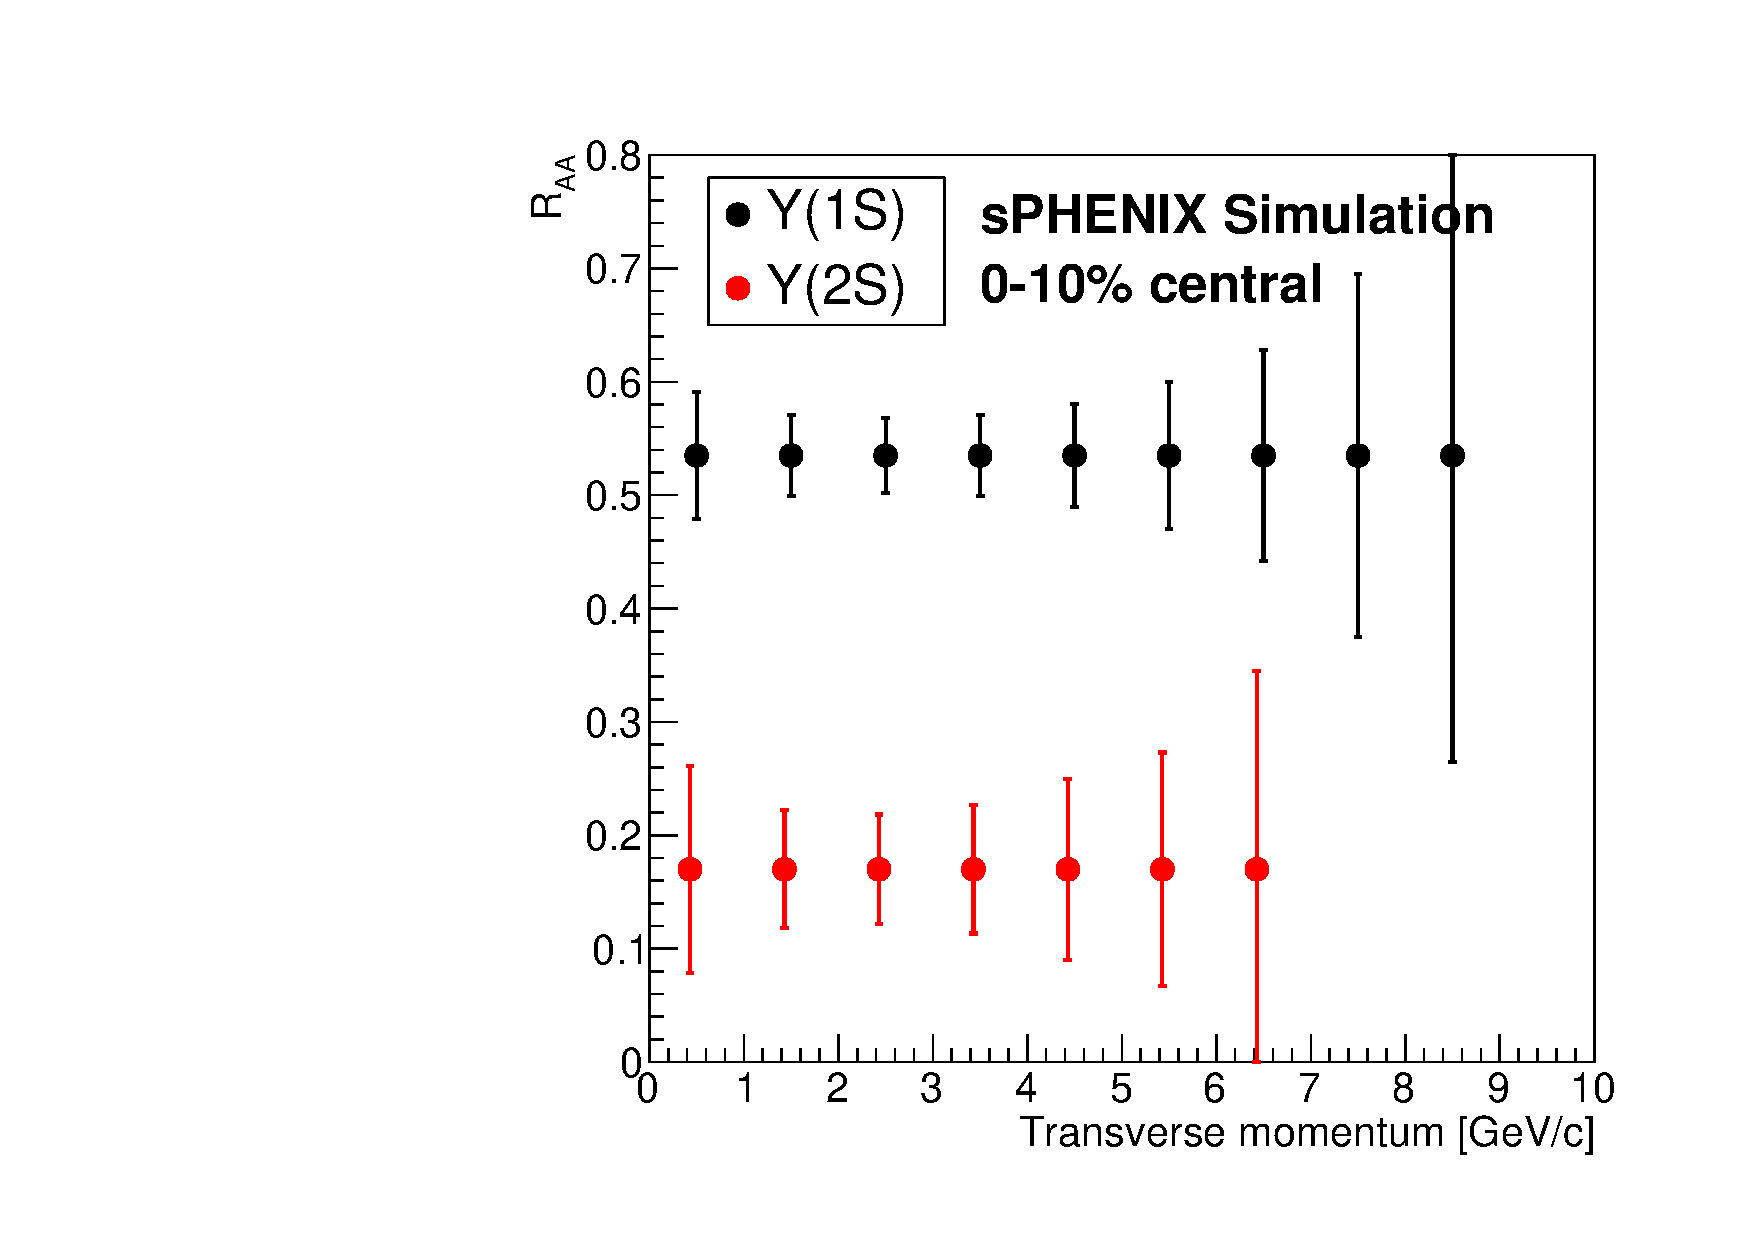
\includegraphics[width=0.55\linewidth]{figs/BUP_Upsilon_RAA_3yr_28wks.pdf}
    \caption{{\textcolor{red}{PLACEHOLDER FIGURE FROM TONY FRAWLEY}}. sPHENIX projected statistical uncertainties, including from background subtraction contributions, for the Upsilon nuclear modification factors from the three-year (2023--2025) proposed run plan.   The projections are assuming the 28 cryo-weeks in each year.
    \label{fig:upsilon3years}}
\end{figure}

\section{Open Heavy Flavor Physics}
\label{sec:HF}

(intro)

\subsection{Diffusion and energy loss of Heavy Quarks in the QGP}


\begin{figure}[htbp]
\centering
% 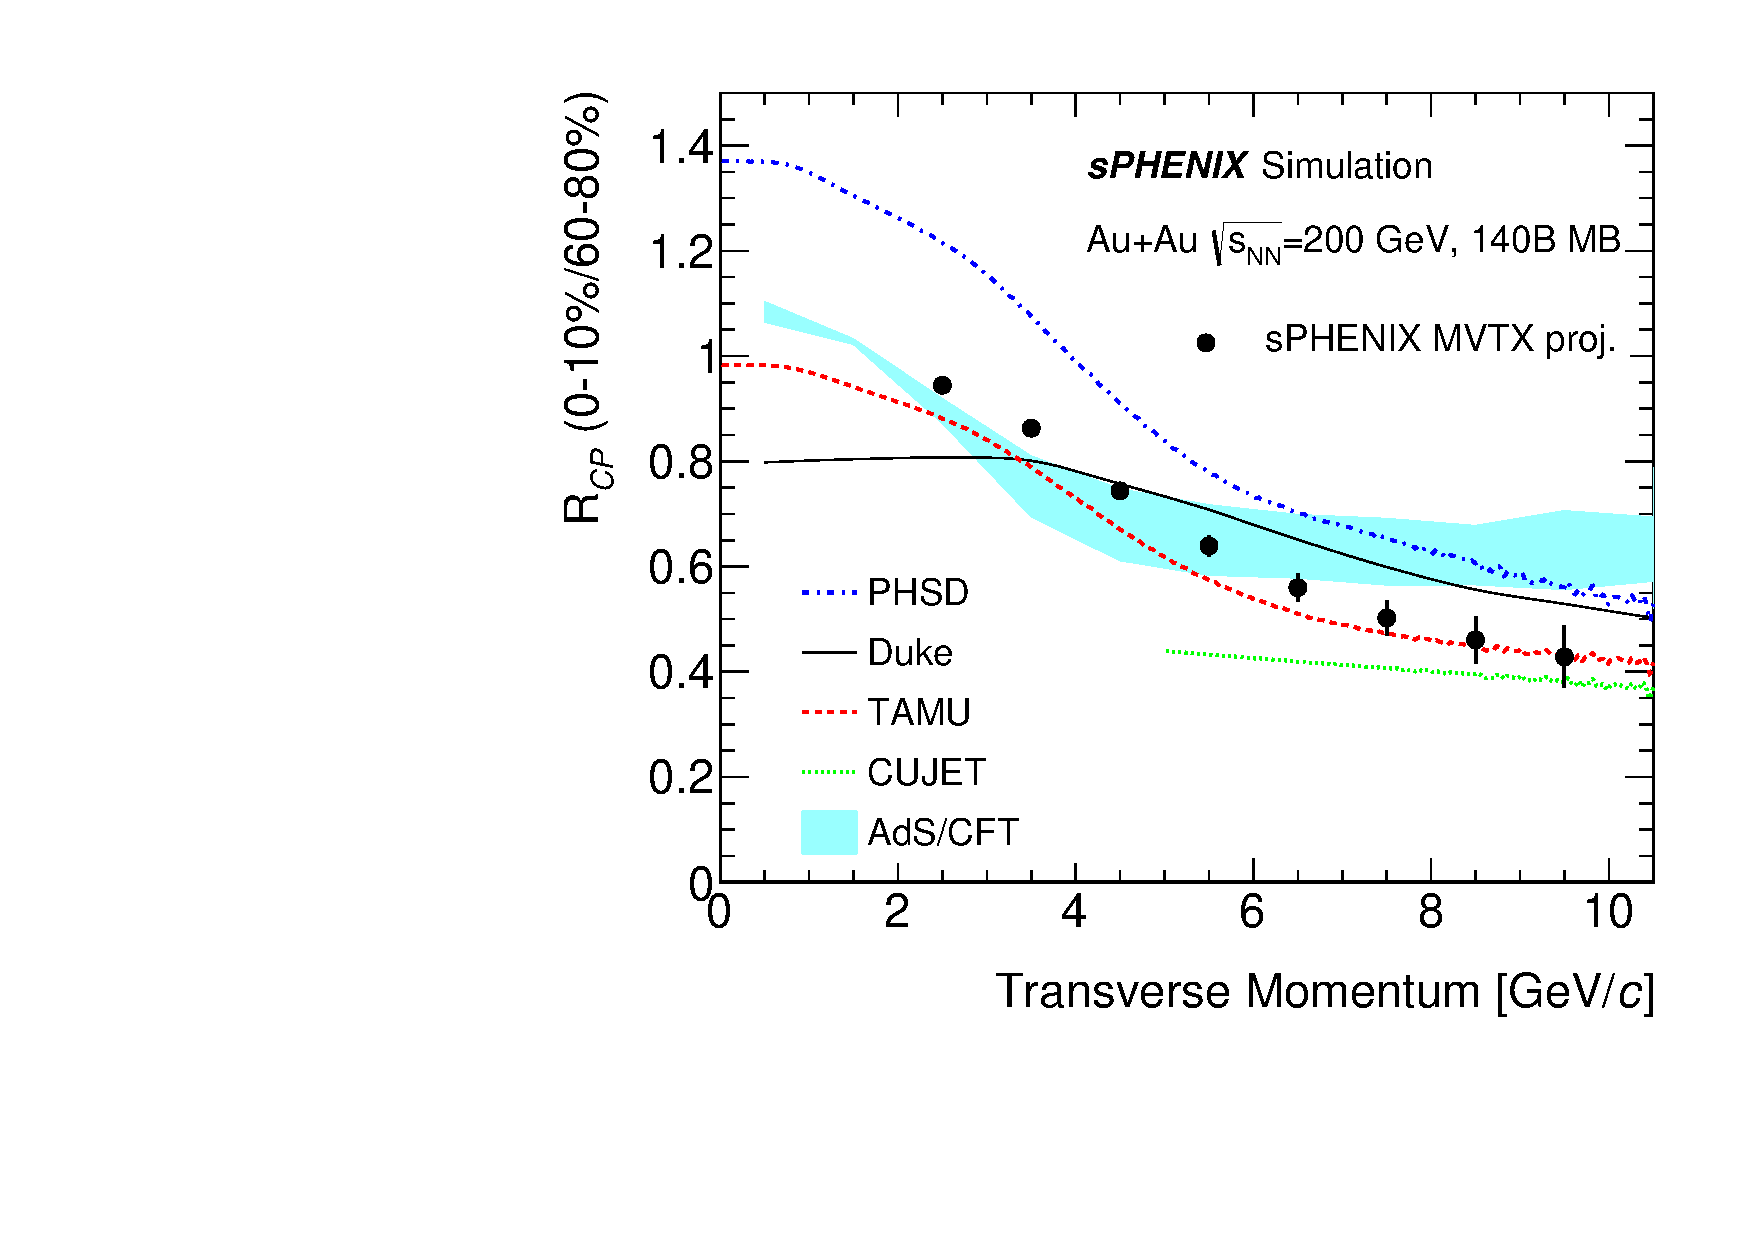
\includegraphics[width=0.48\textwidth]{figs/Rcp_proj_140B_theory.pdf}
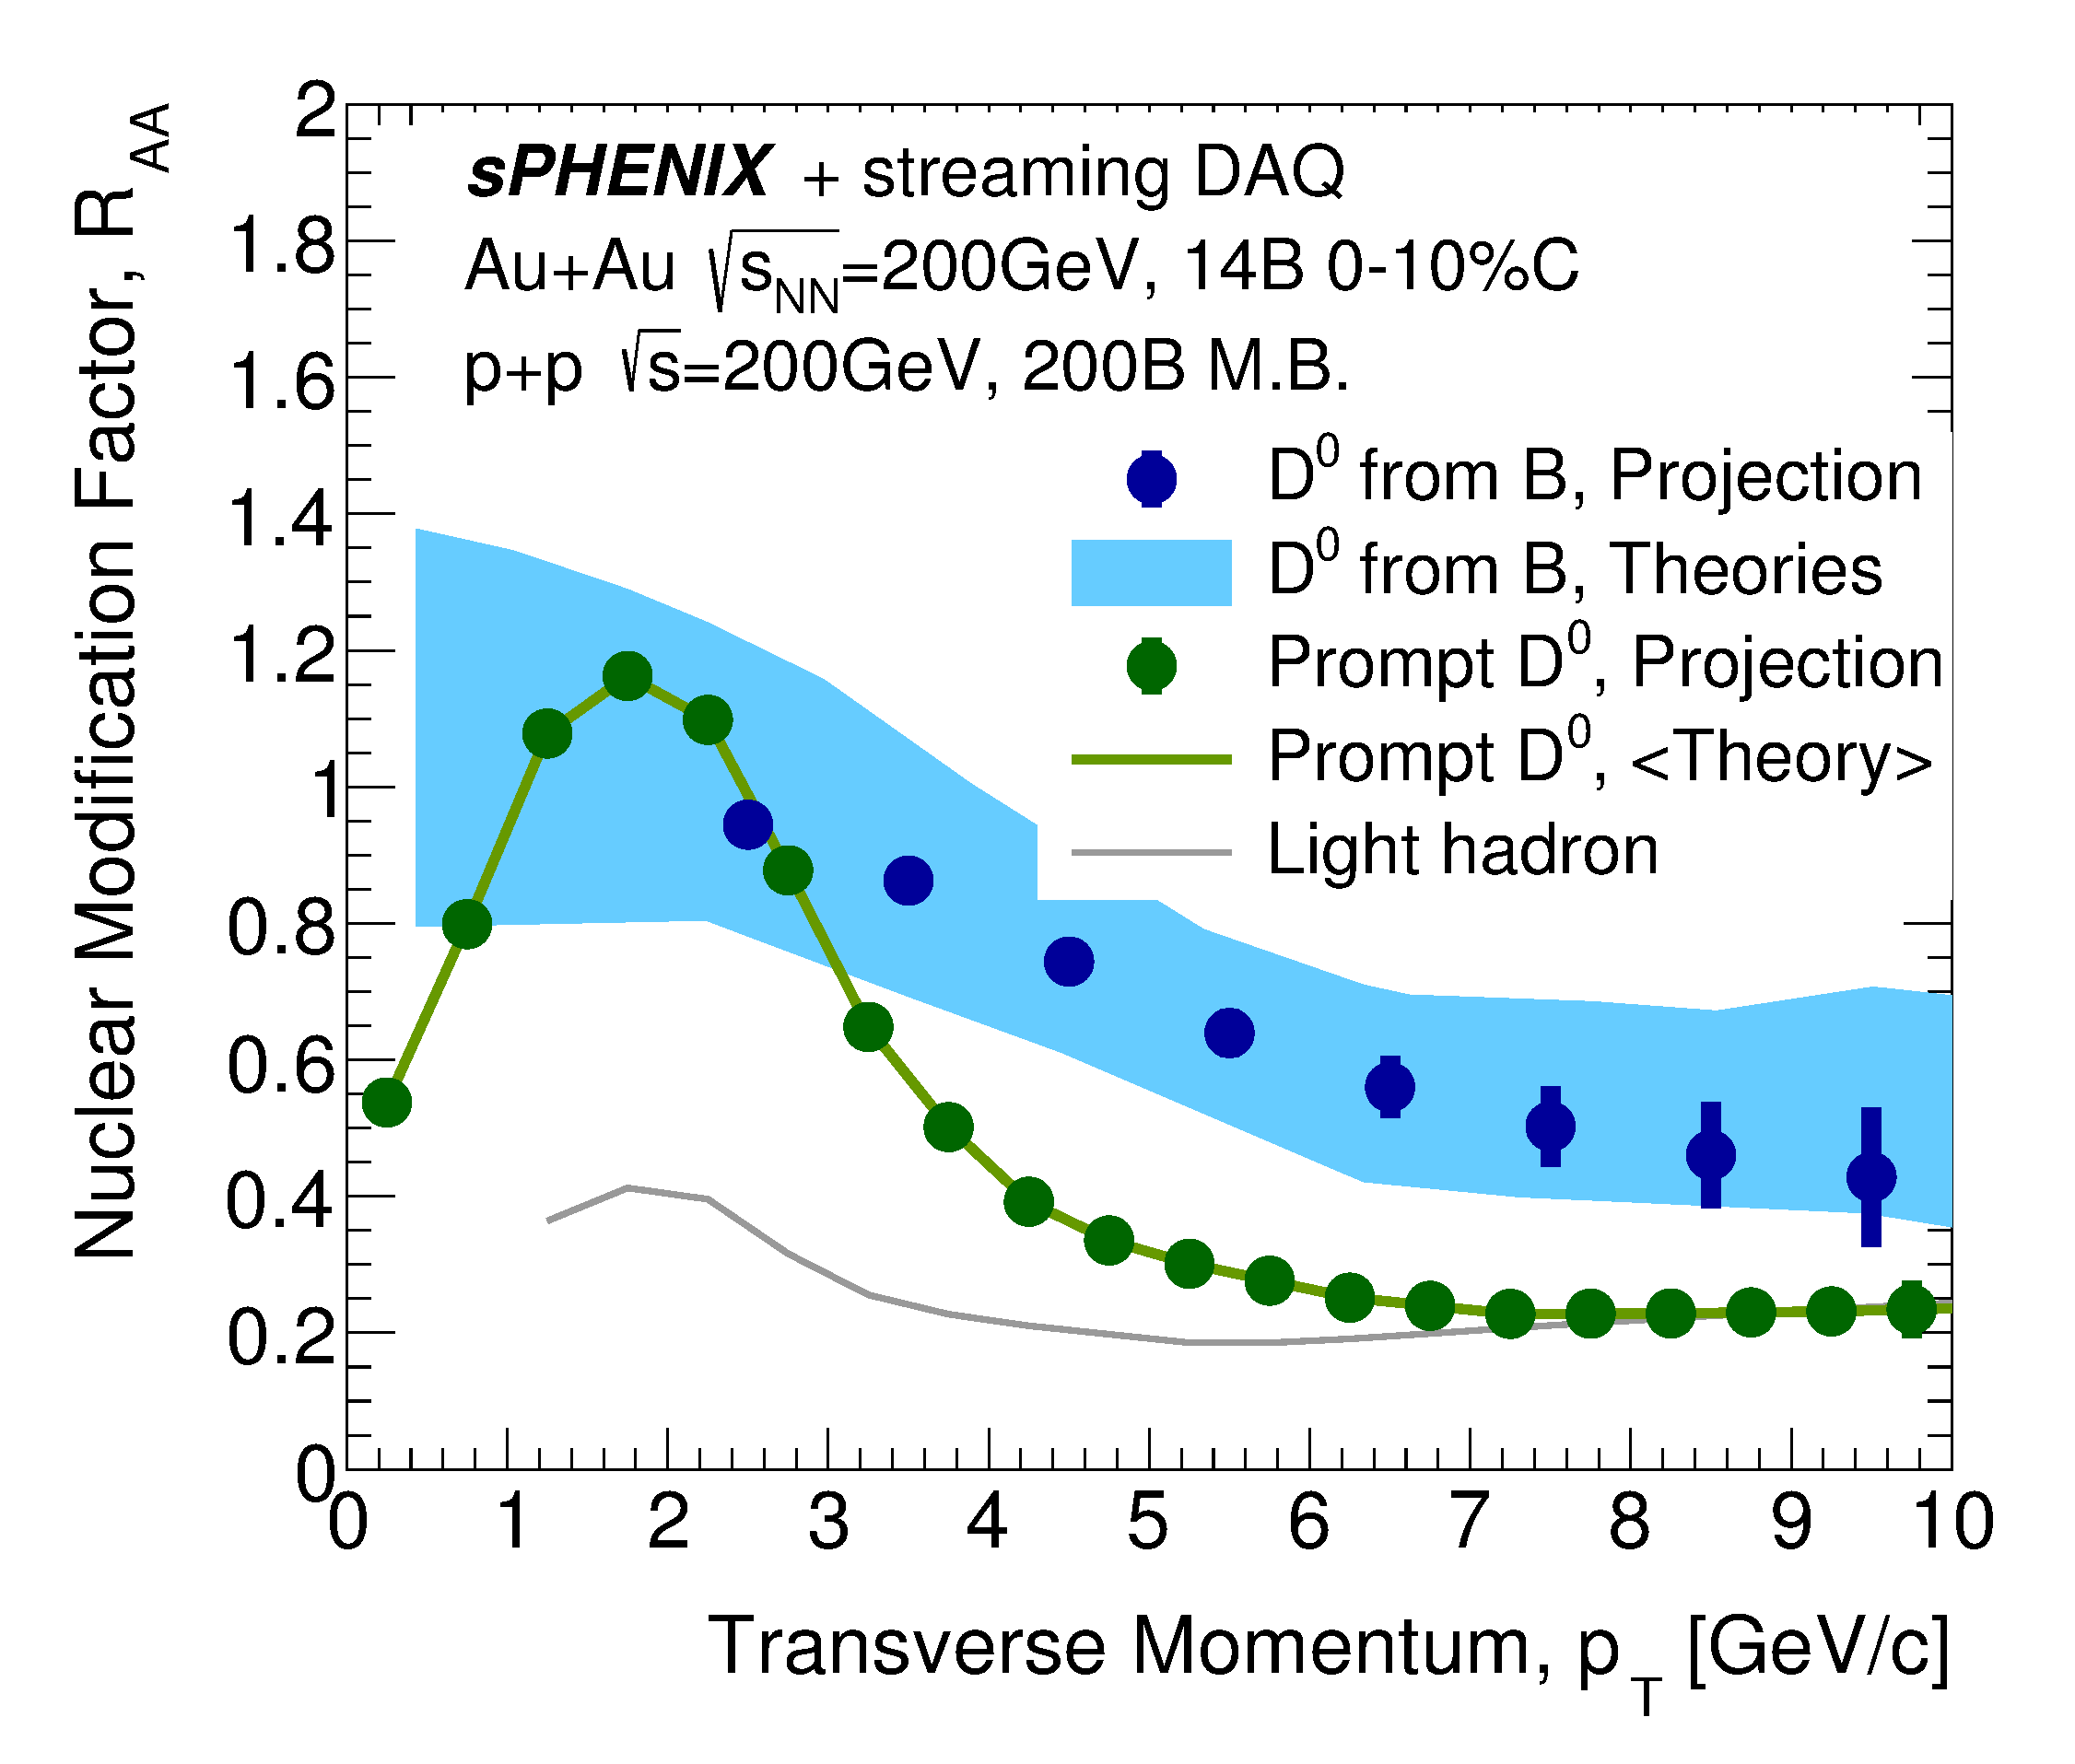
\includegraphics[width=.49\linewidth]{figs/RAA_DB_theory_root_RAADB_pp200B.pdf}
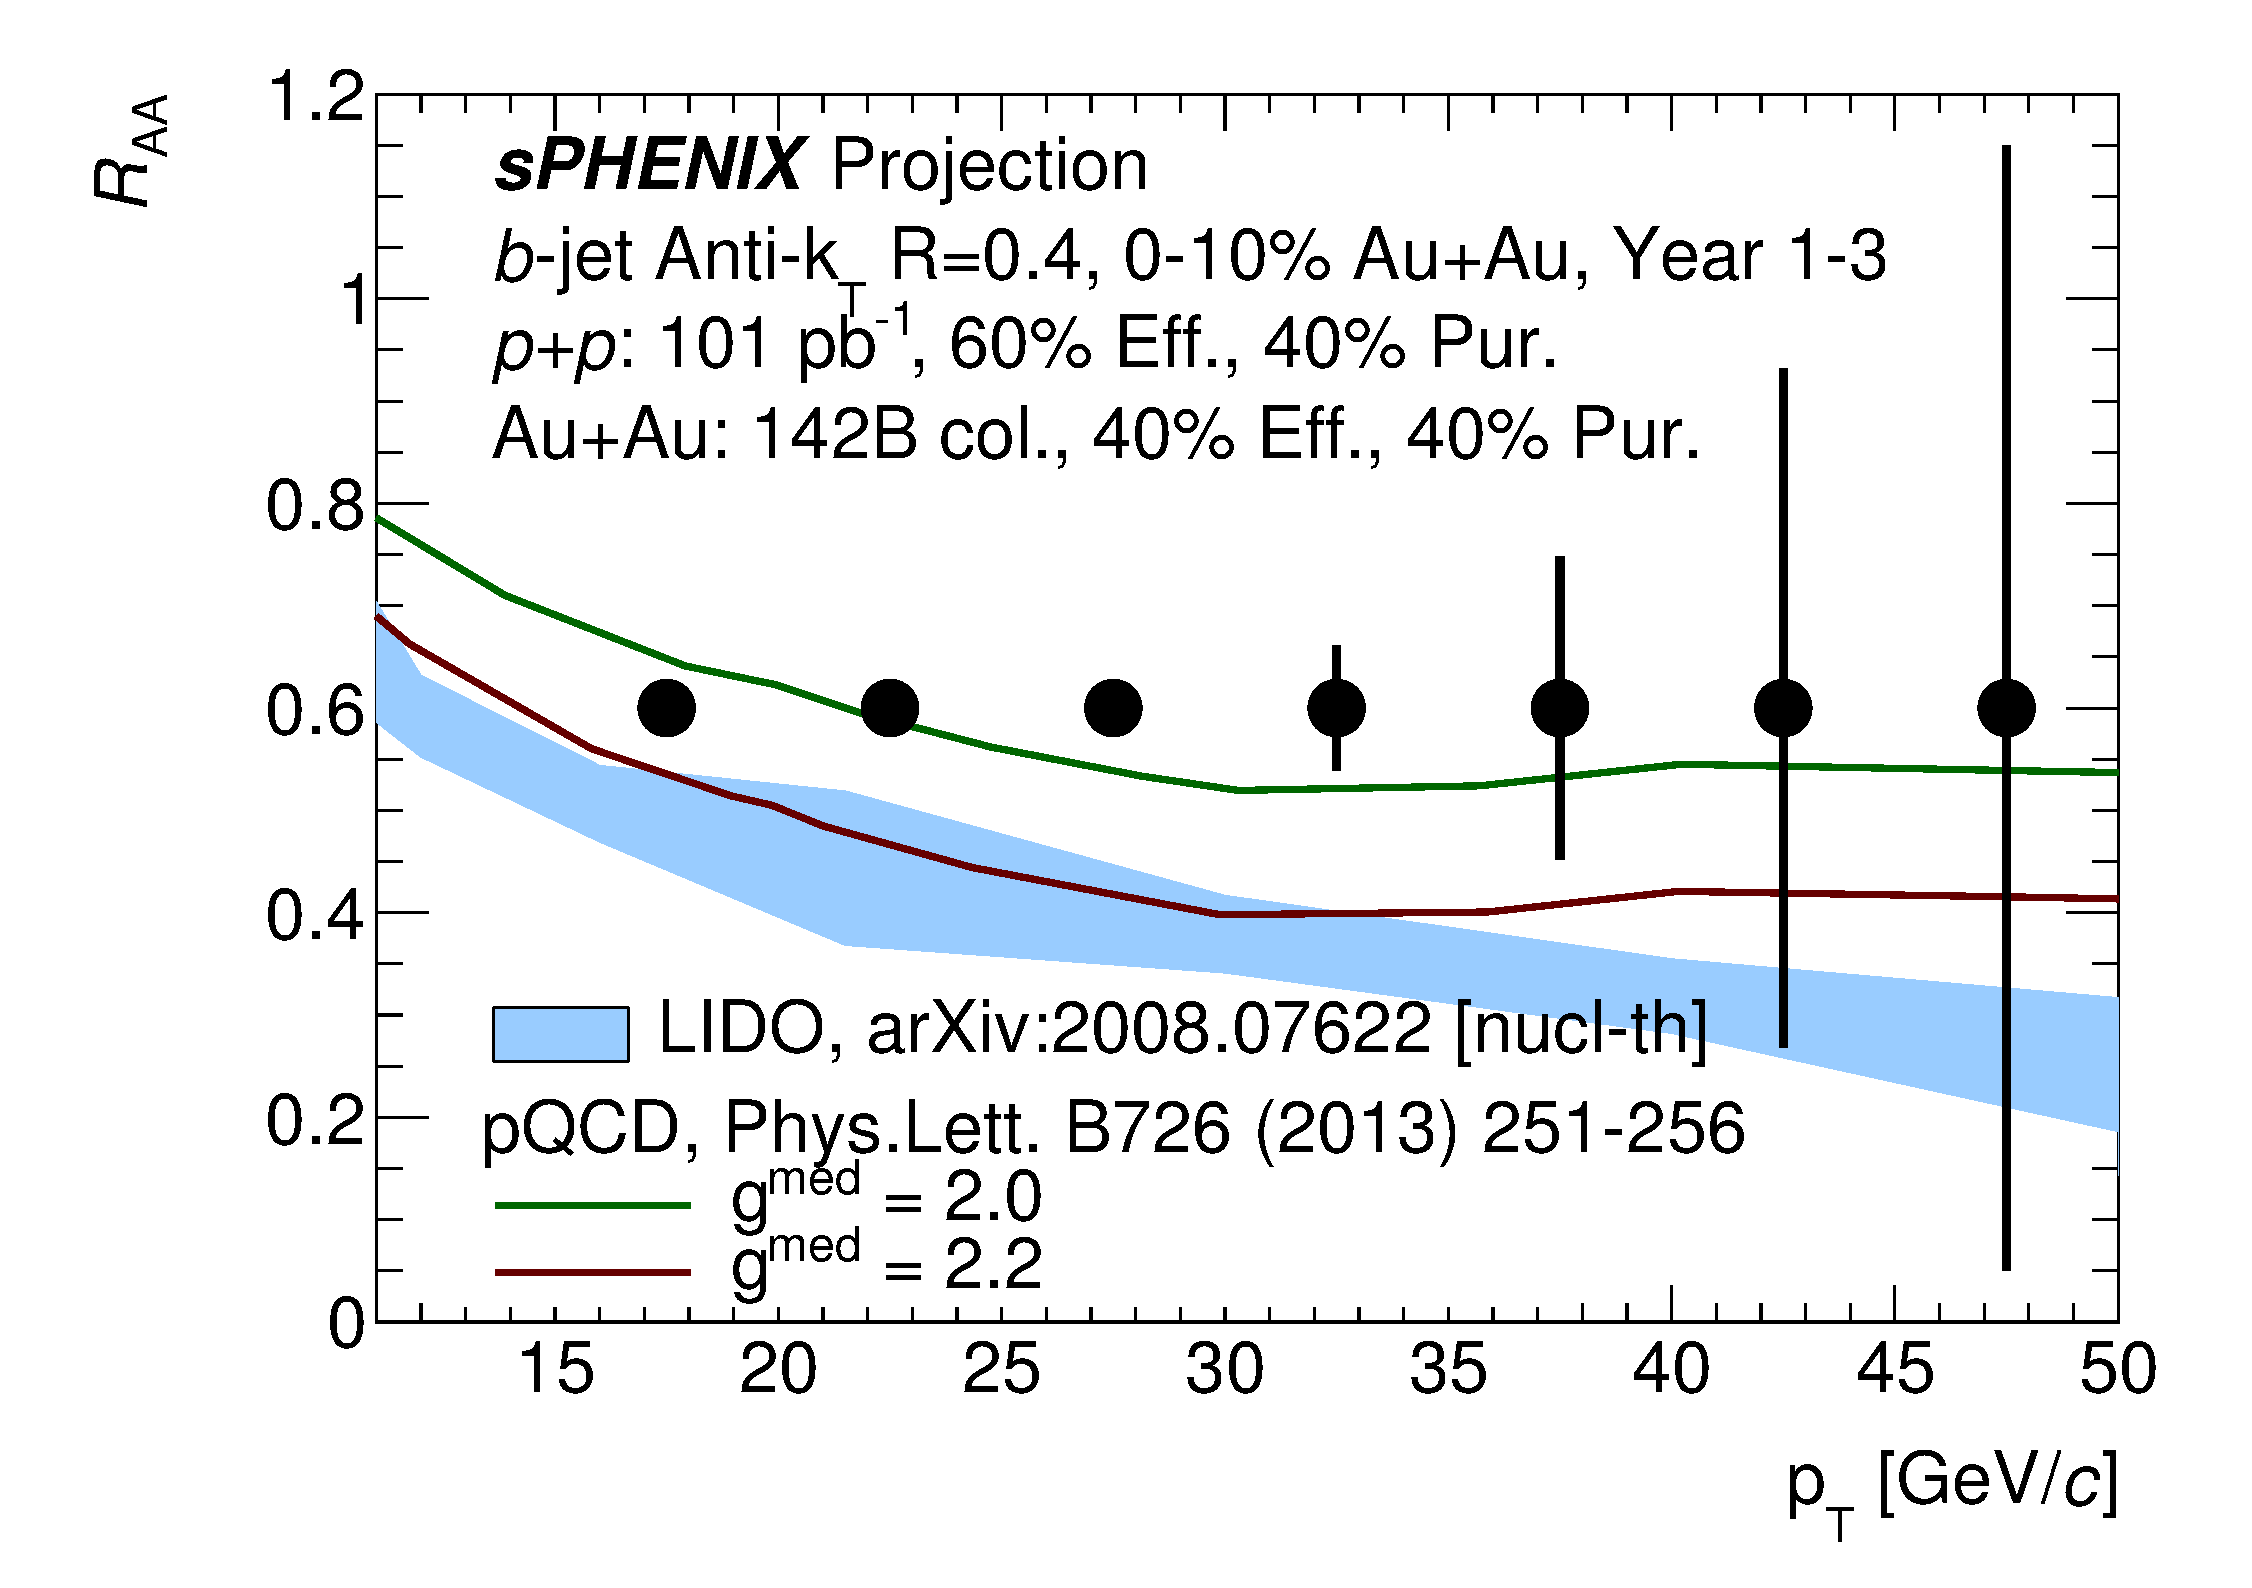
\includegraphics[width=0.5\textwidth]{figs/200pp_pythia8_CTEQ6L_7GeV_ALL_cfg_eneg_DSTReader_root_Draw_HFJetTruth_CrossSection2RAA_Theory_3yr_deta0_70.pdf}
\caption{Projected statistical uncertainties of nuclear modification factor $R_{cp}$ and \raa measurements of non-prompt/prompt $D^0$ mesons (left) and $b$-jet (right) as a function of \pT in 0--10\% central \auau collisions at $\sqrt{s_{NN}}=200$~GeV from a dataset of 140 billion minimum bias \auau collisions expected from the three-year sPHENIX operation. Left: the solid blue and red lines are best fit to the RHIC data, the solid black line is from a model calculation for B mesons and the dotted line is the theory calculation for $D$-mesons coming from $B$-meson decays. Right: the solid and dashed lines are from model calculations with two different coupling parameters to the QGP medium, $g^{\textrm{med}}$, and the statistical projection is based on the assumption of $\raa =0.6$. sPHENIX will enable these highest precision $B$-meson measurement and the first heavy flavor jet measurement at RHIC, which will place stringent tests on models describing the coupling between heavy quarks and the QGP~\cite{Huang:2013vaa,Duke,TAMU,PHSD,CUJET}}
\label{fig:HF-inclusive-RAA}
\end{figure}

\begin{figure}[htbp]
\centering
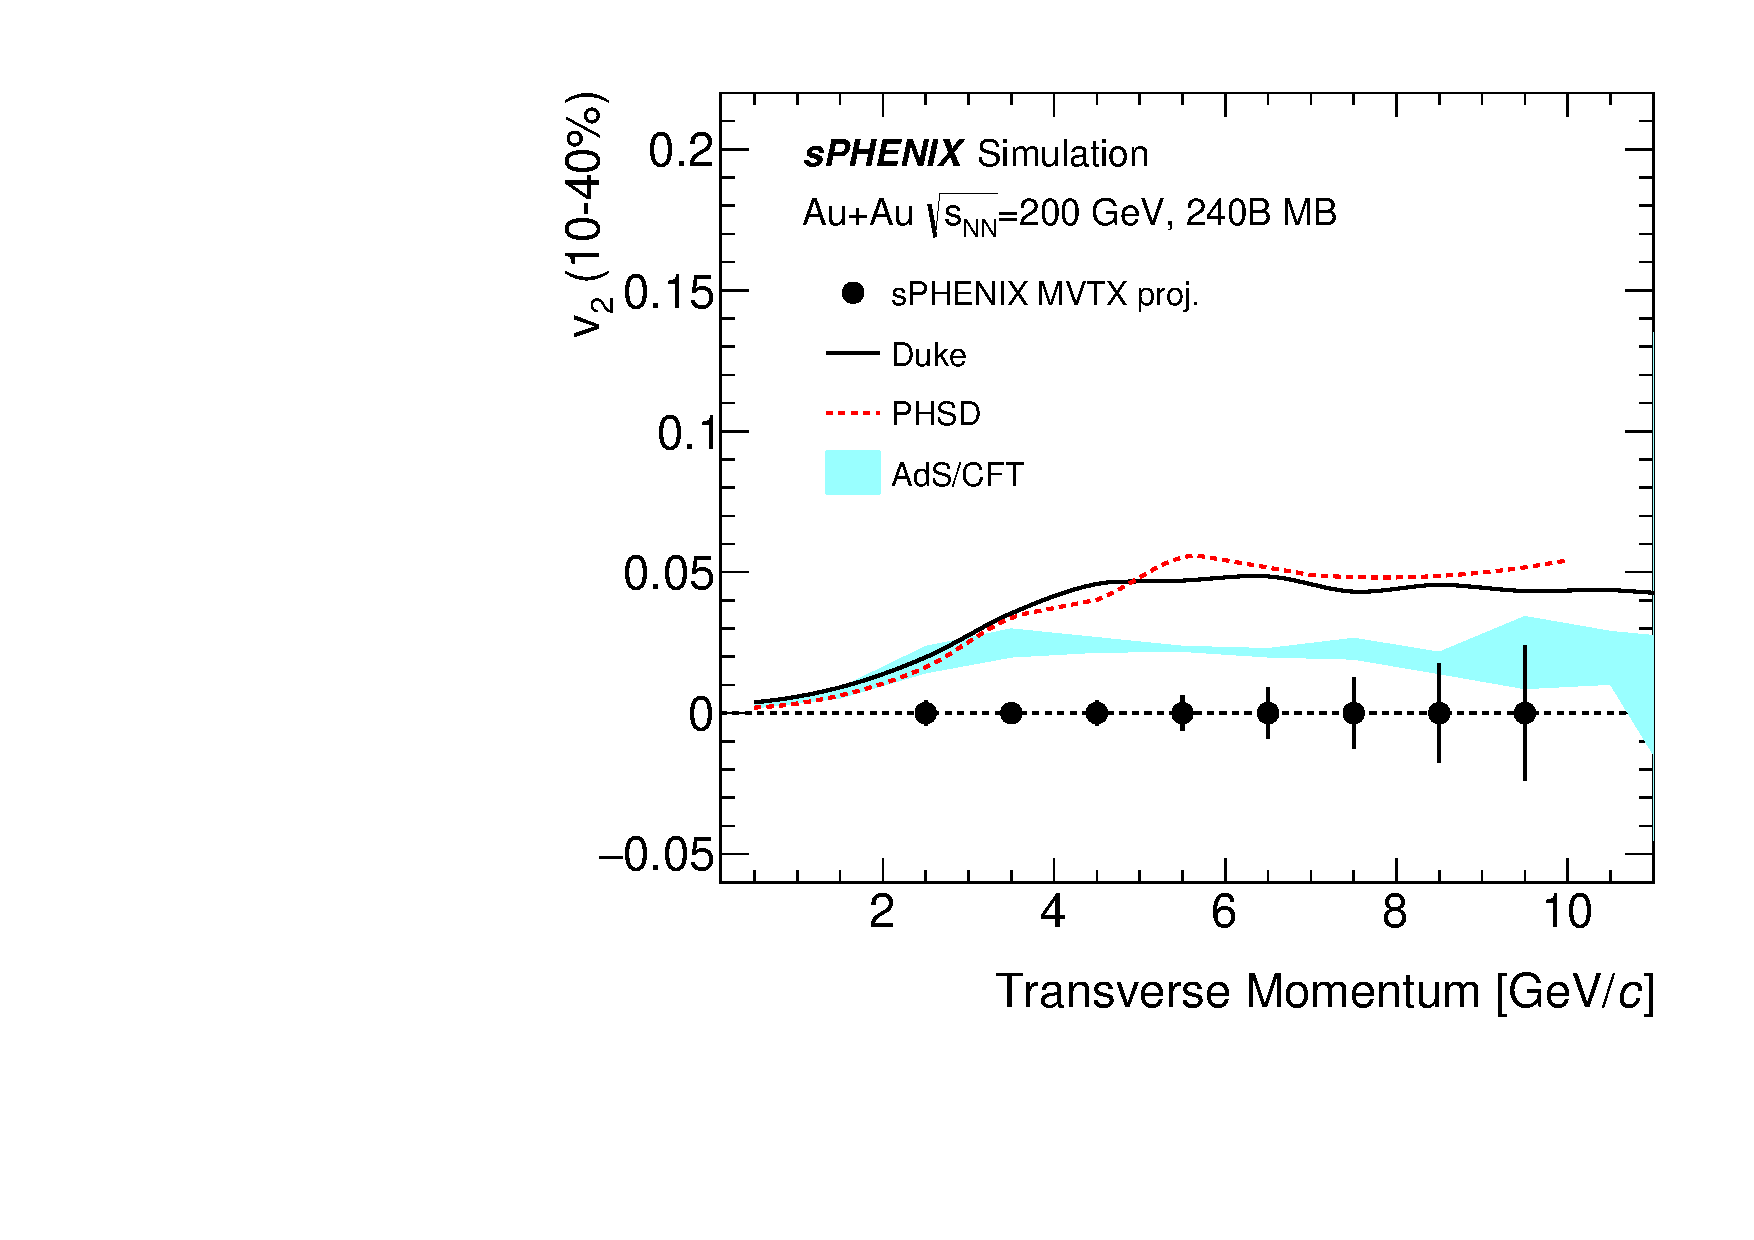
\includegraphics[width=0.48\textwidth]{figs/v2_proj_240B_theory.pdf}
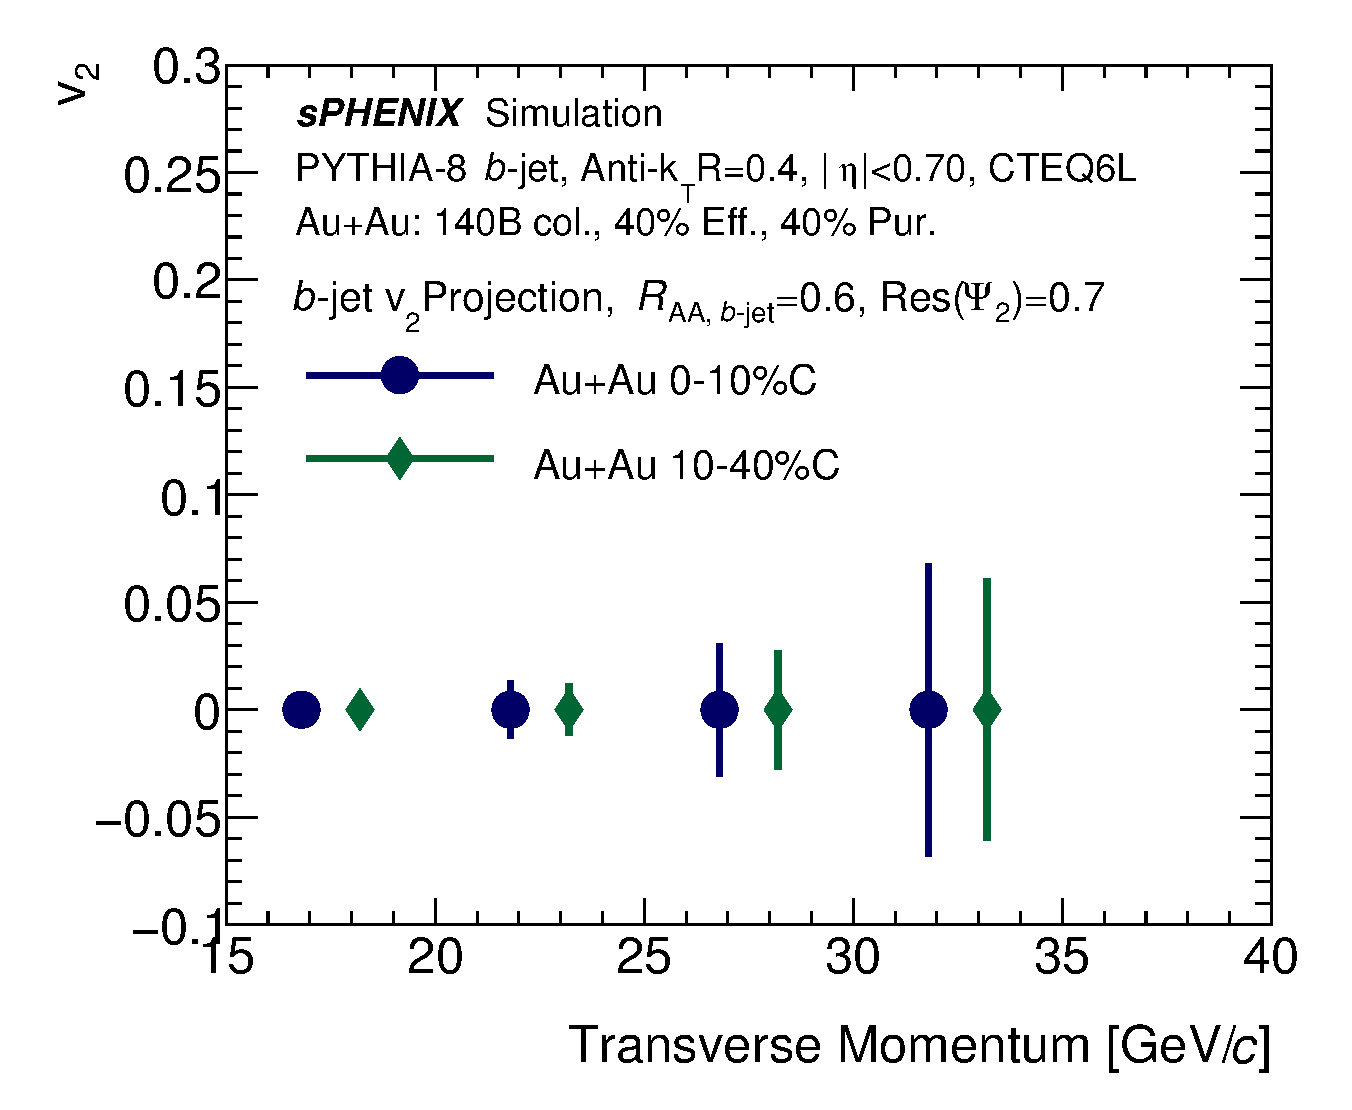
\includegraphics[width=0.5\textwidth]{figs/200pp_pythia8_CTEQ6L_7GeV_ALL_cfg_eneg_DSTReader_root_Draw_HFJetTruth_CrossSection2v2_3yr_EPR0_7_deta0_70.pdf}
\caption{Projected statistical uncertainties of $v_2$ measurements of non-prompt/prompt $D^0$ mesons (left) and $b$-jets (right) as a function of \pT in 10--40\% central \auau collisions at $\sqrt{s_{NN}}=200$~GeV from a dataset of 140 billion minimum bias \auau events expected from the three-year sPHENIX operation.  Left: the blue dotted line is from best fit of RHIC data, and the black line is for $B$-meson assuming $m_T$ scaling in $v_2$. \cite{Adamczyk:2017xur, Duke, TAMU, PHSD}}
\label{fig:HF-v2}
\end{figure}


\begin{figure}[htbp]
\centering
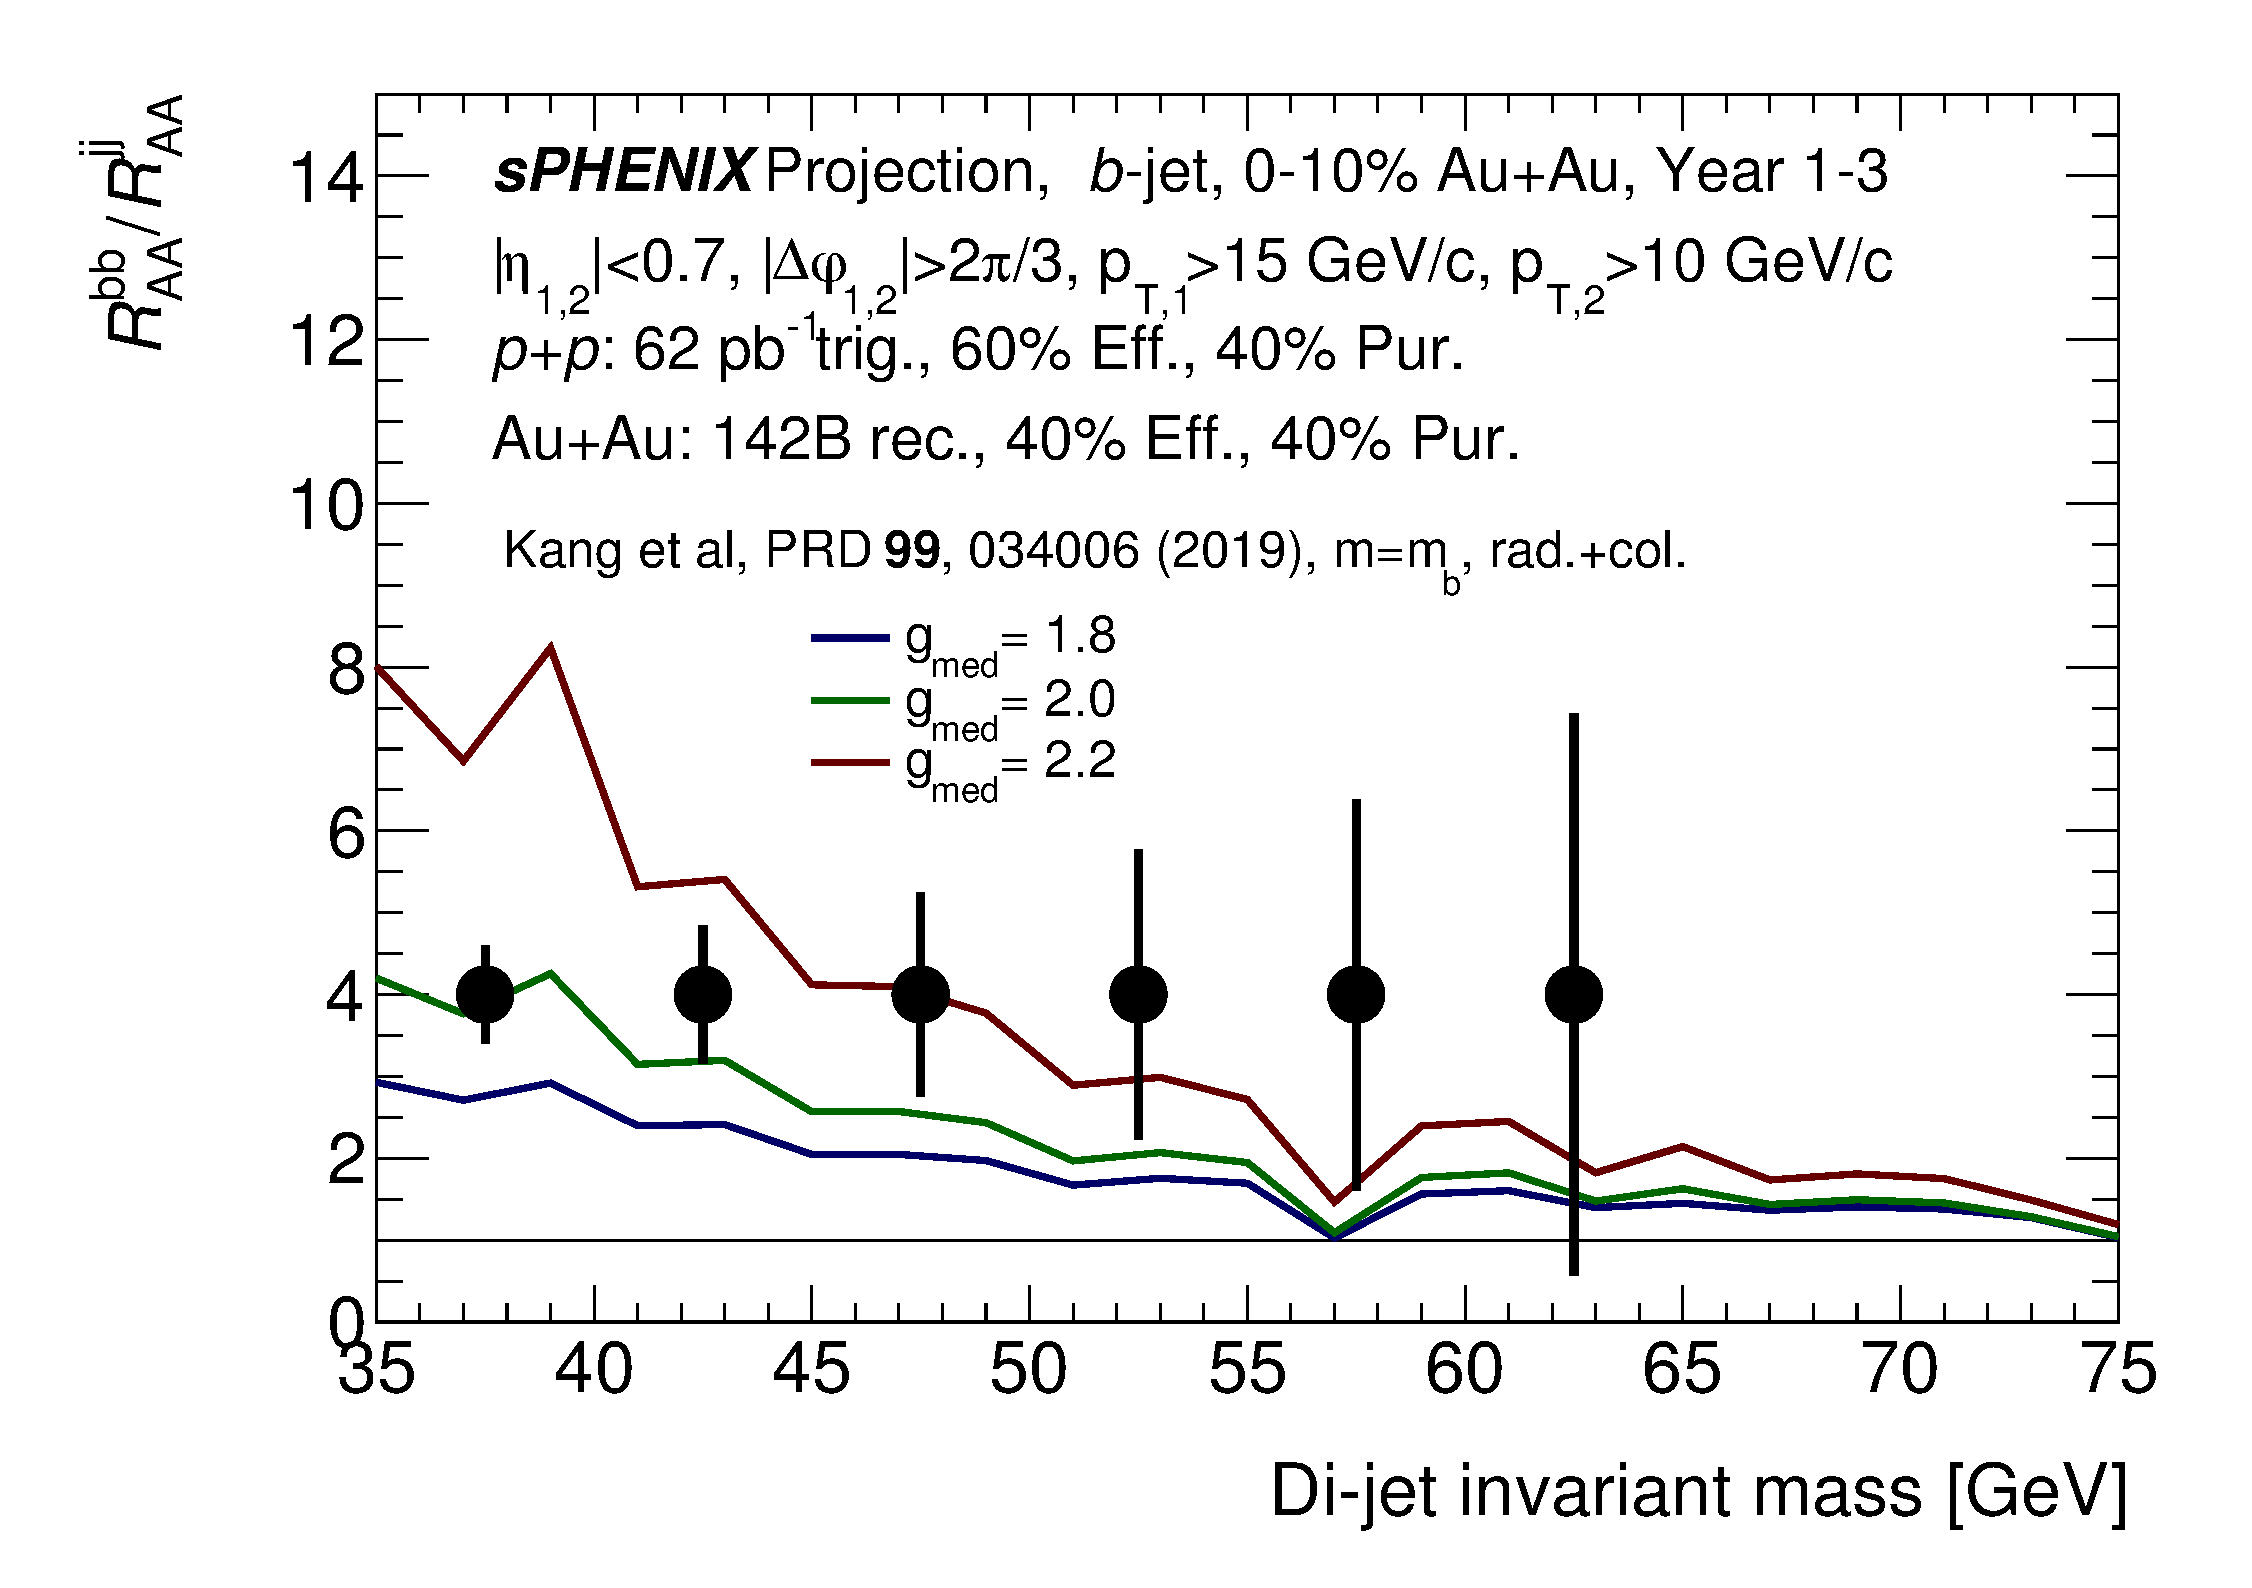
\includegraphics[width=0.48\textwidth]{figs/200pp_pythia8_CTEQ6L_7GeV_ALL_cfg_eneg_DSTReader_root_Draw_HFJetTruth_InvMass_CrossSection2RAARatio_Theory_3yr_deta0_70.pdf}
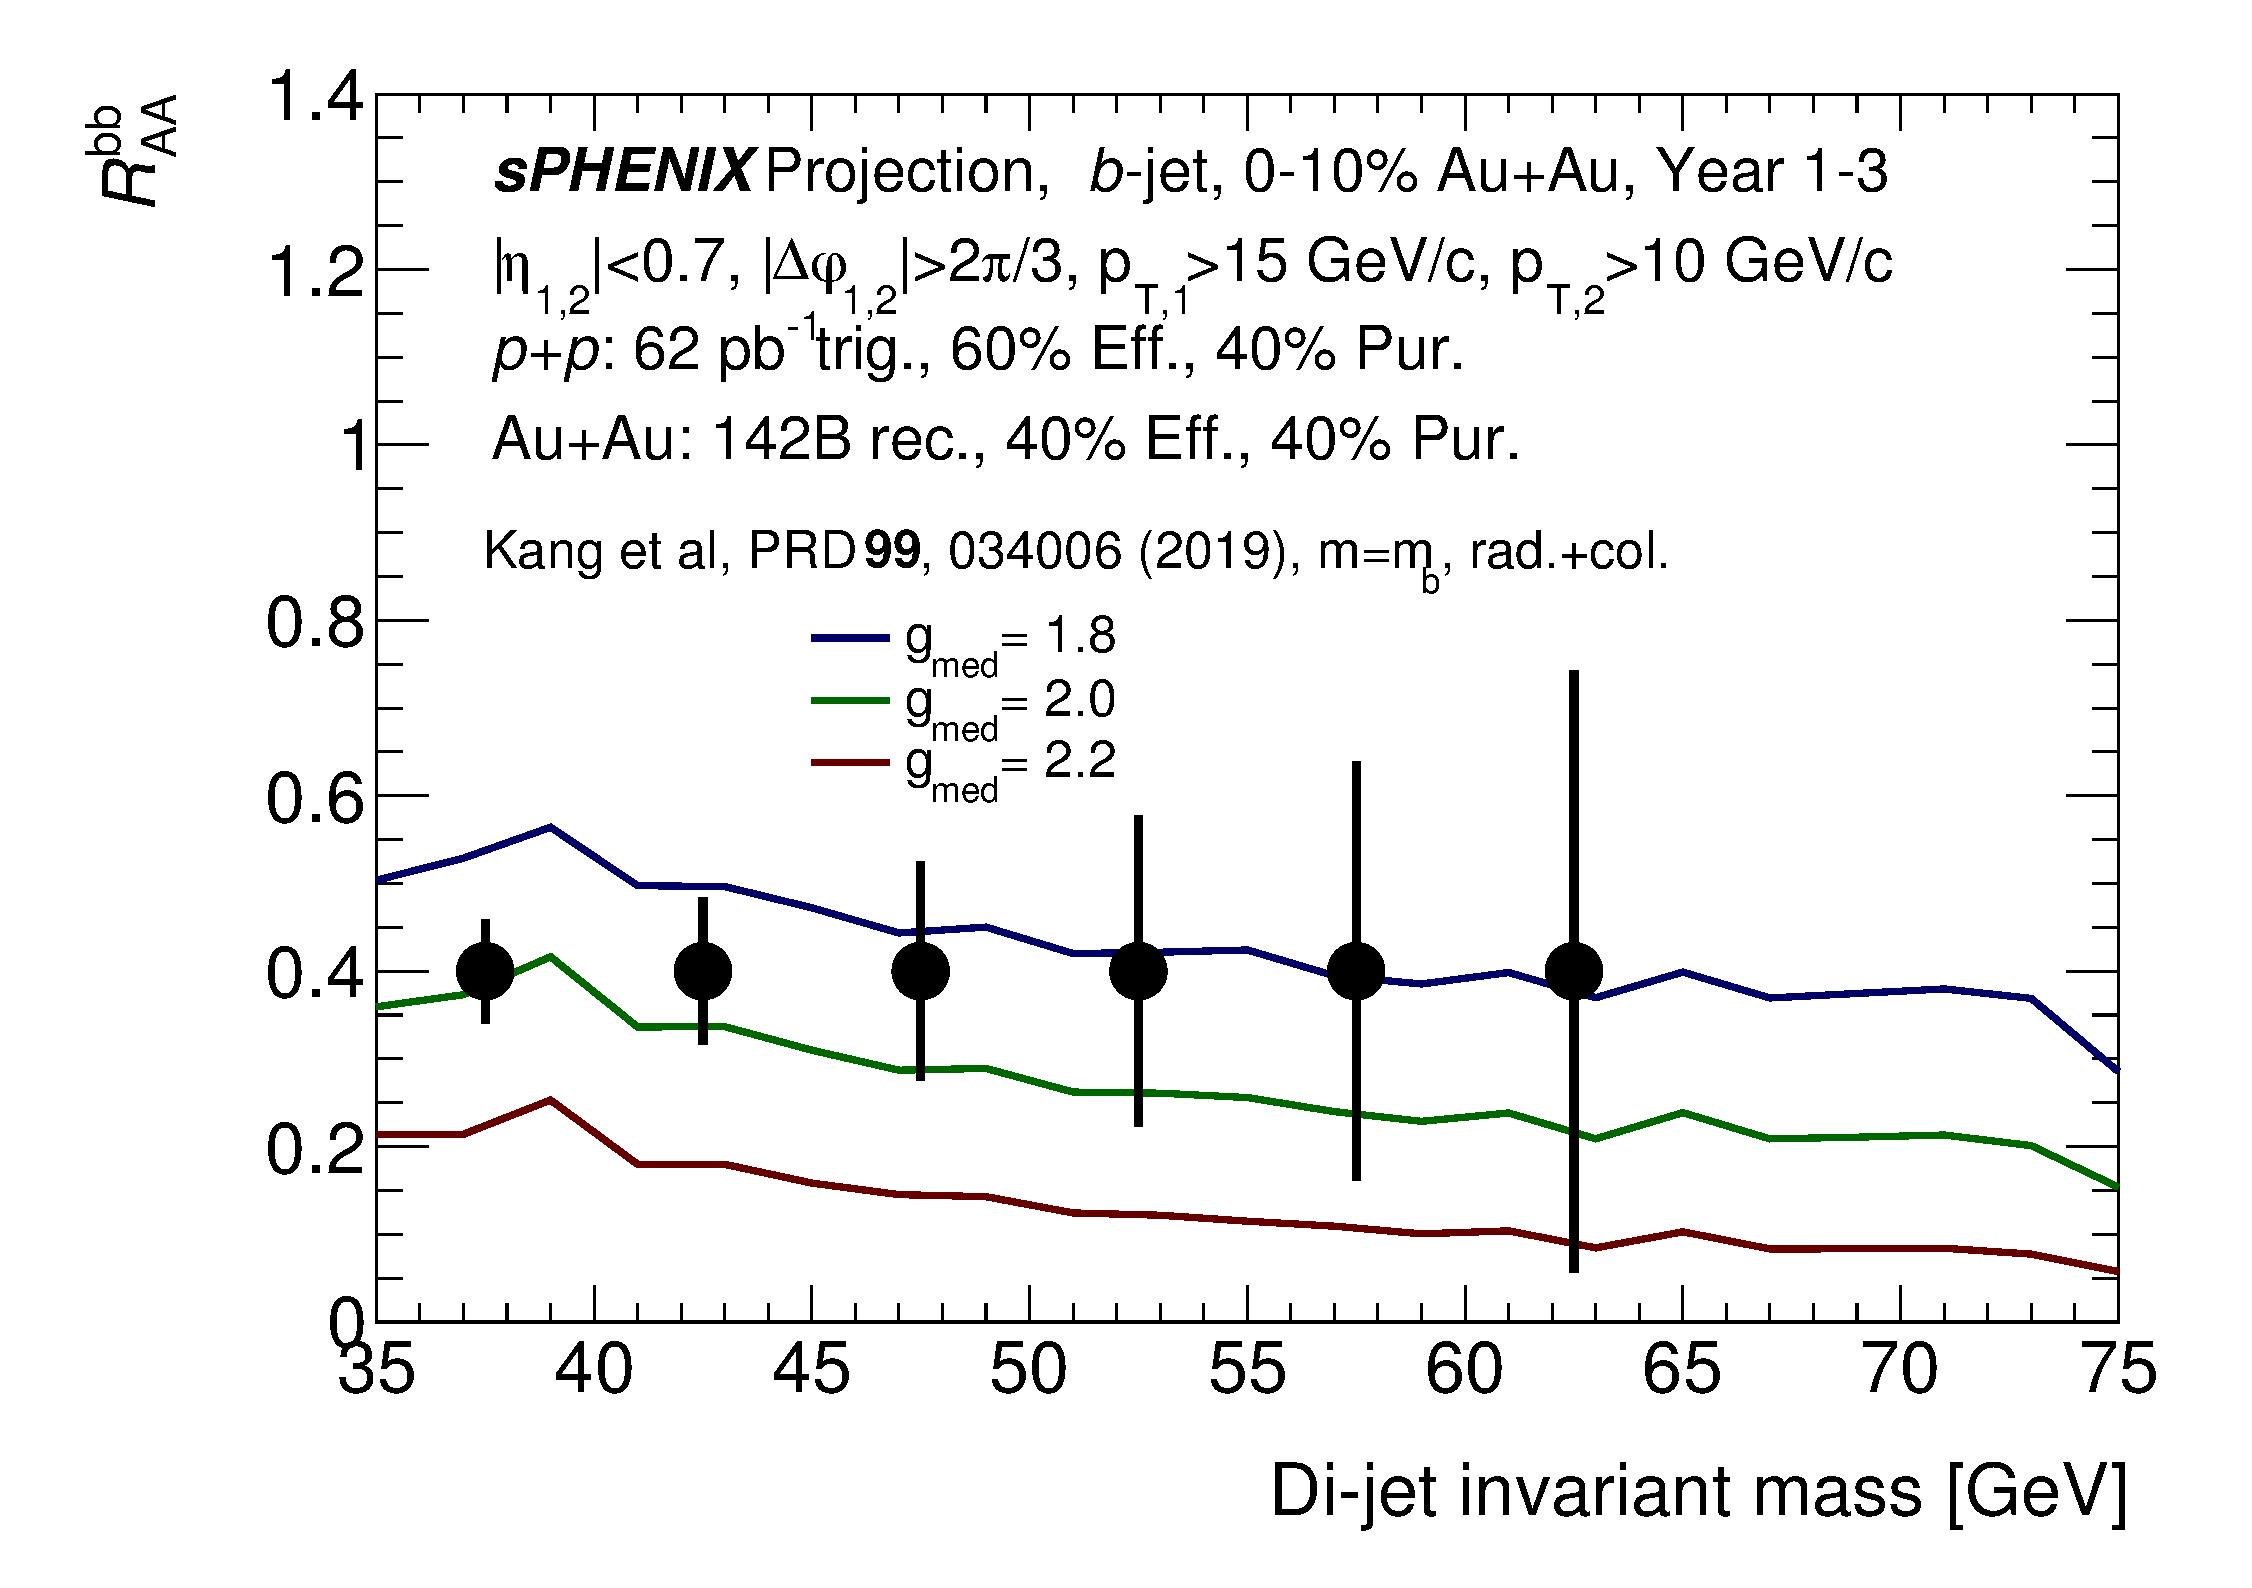
\includegraphics[width=0.5\textwidth]{figs/200pp_pythia8_CTEQ6L_7GeV_ALL_cfg_eneg_DSTReader_root_Draw_HFJetTruth_InvMass_CrossSection2RAA_Theory_3yr_deta0_70.pdf}
\caption{Projected statistical uncertainties of nuclear modification for $b$-jet pairs and $b$-jet-light-jet super-ratio.}
\label{fig:HF-bjet-pair}
\end{figure}


% \begin{figure}[htbp]
% \begin{center}
% 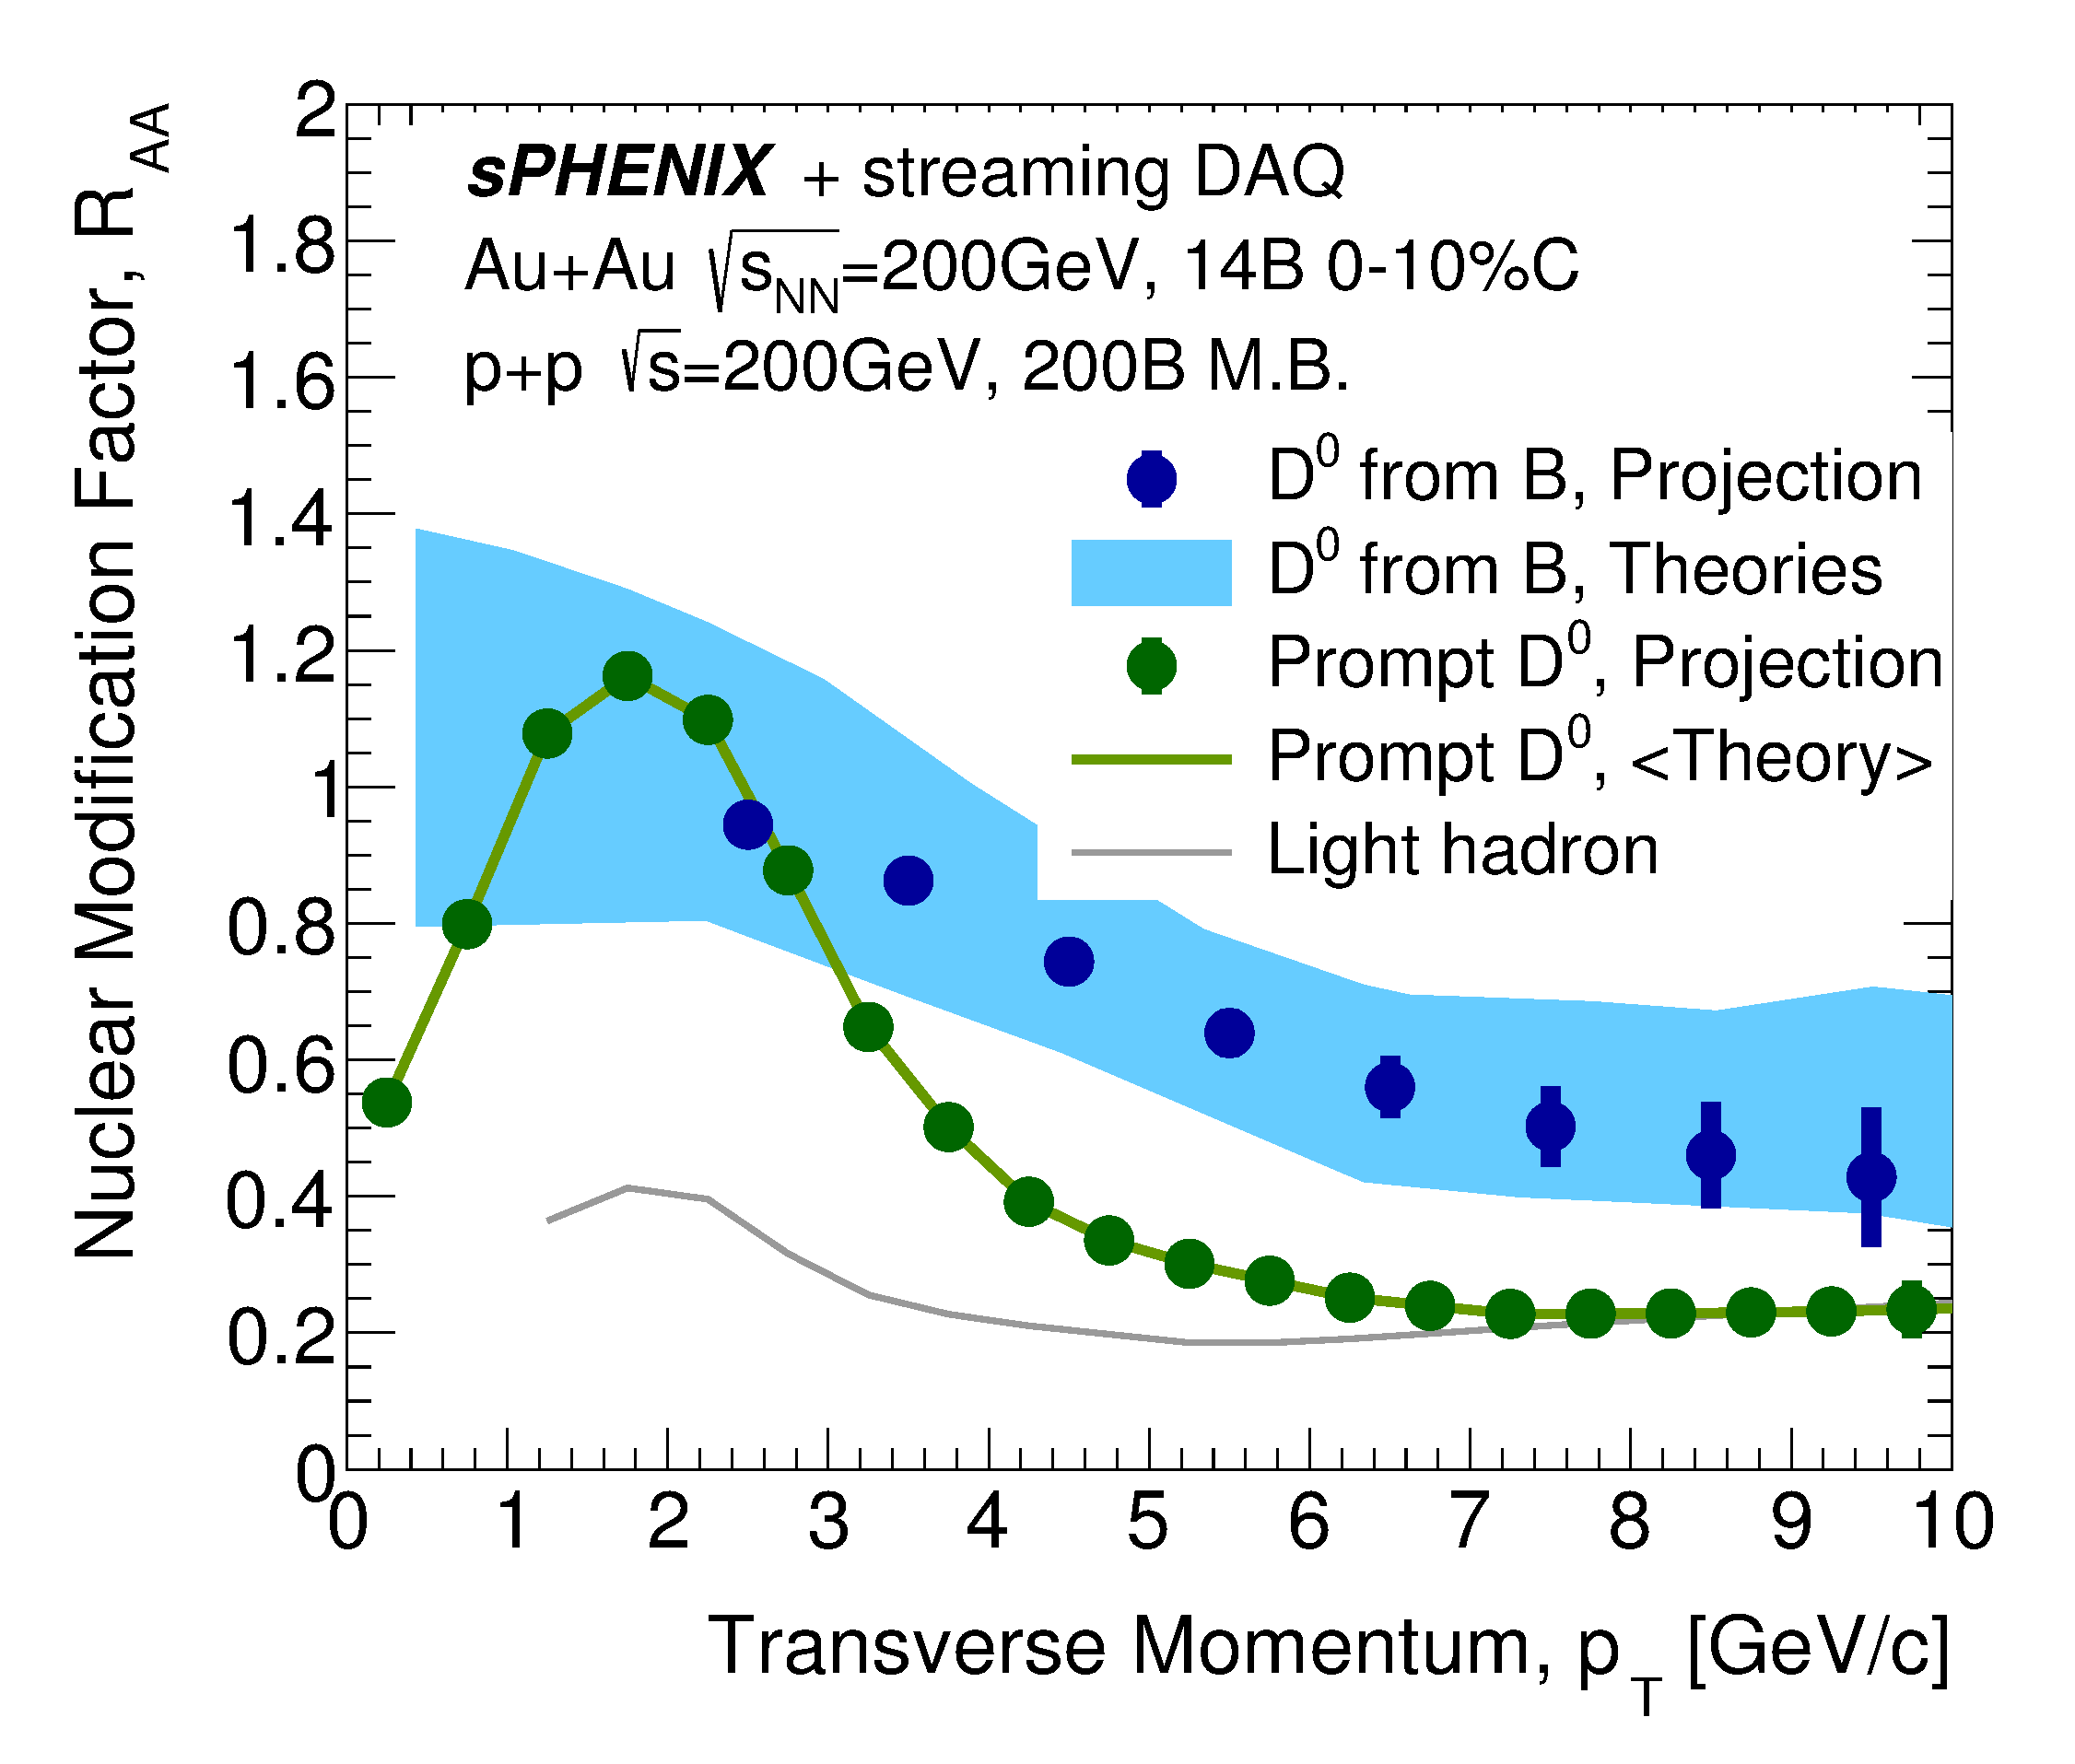
\includegraphics[width=.49\linewidth]{figs/RAA_DB_theory_root_RAADB_pp200B.pdf}
% % 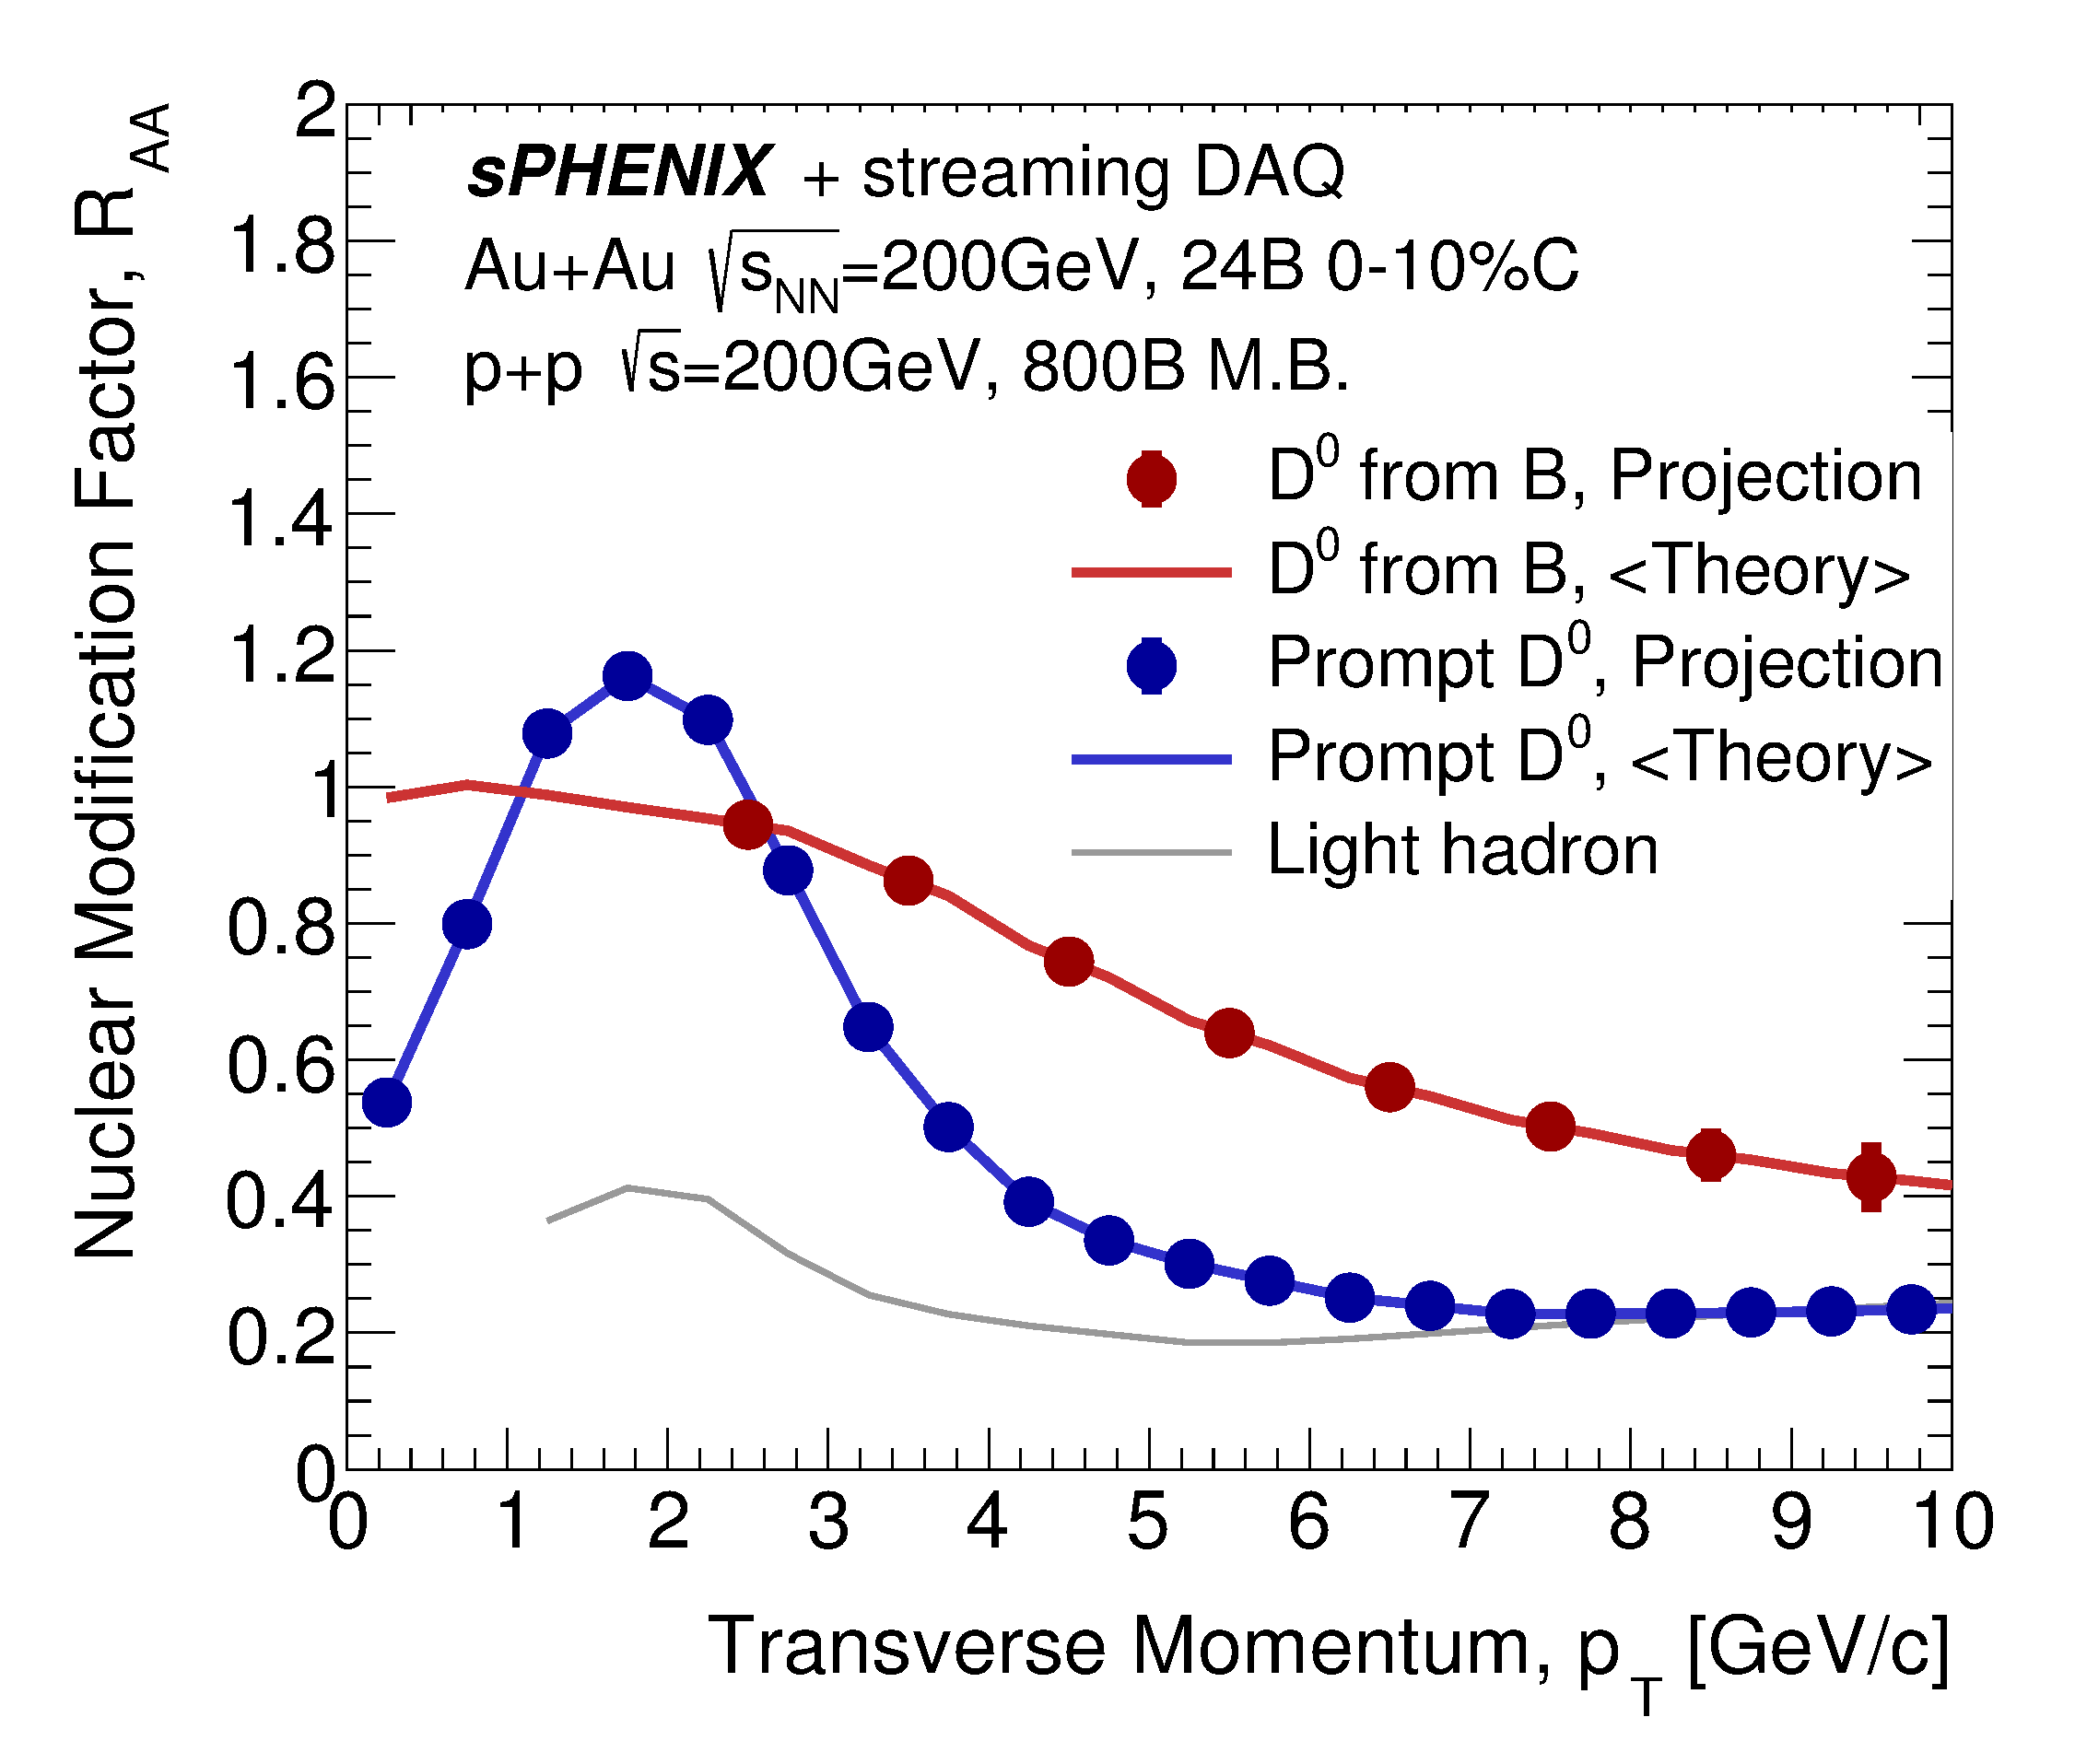
\includegraphics[width=.49\linewidth]{figs/RAA_DB_theory_root_RAADB.pdf}
% \caption{Statistical projections of $R_AA$ for $D^0$ from $B$ decays for Year-2 data taking.}
% \label{fig:RAA-D0}
% \end{center}
% \end{figure}


(Moved from streaming readout section, need rewritten....)
The currently envisioned sPHENIX experiment is designed to take large statistics of calorimeter triggered events in the \pp collisions, which will sample 2 trillion delivered \pp collisions in the vertex acceptance of the silicon tracker (18\% of all collisions)~\cite{something}. For observables that utilize calorimeter for analysis, a trigger can usually be designed, such as leptonic decays at higher $p_T$, jets, photon, and their correlation observables. However, low-$p_T$  ($<10$~GeV$/c$) HF hadrons usually decay hadronically and leave relatively low signals in the calorimeters when compared with the underlying event. Therefore, they cannot be efficiently collected via calorimeter triggers, which have a hadron energy threshold of 10 GeV. Therefore, in the currently envisioned sPHENIX detector, there is no efficient way in triggering such events in the \pp collisions. And in the 15 kHz sPHENIX trigger bandwidth, one would only reasonable request around few kHz of the minimum bias \pp trigger for this new program. Assuming 50\% vertex range selection purity , 1 kHz M.B. trigger leads to recording $2\times10^{-4}$ of the delivered luminosity . This translates to quite limited statistics for these rare low-$p_T$ HF signals as quantified in Table X [Need table].
This upgrade carries out the upgrade enabling the collection of a sufficient amount of minimum bias \pp events. That is 10\% delivered luminosity (see next Chapter), 200 billion events in vertex tracker acceptance, which is a factor of 500 improvements. This dataset enables a comprehensive low-$p_T$ hadron program as discussed in this subsection. The analysis for these HF hadronic channels does not require calorimeter information. Instead, they can be identified with the precision tracking detectors of sPHENIX (at $p_T$=5 GeV$/c$, $\sigma(p)/p=1\%$, $\sigma(DCA)<10$~$\mu$m ) via a combination of decay topology and invariant mass, as demonstrated for even the busiest events of Au+Au collisions through detailed simulation studies in~\cite{something}. 
 
The non-prompt $D^0$ meson production is a clean channel to access b-quark via its decay chain. Using tracker data alone, both prompt and non-prompt $D^0$ can be reconstructed via the invariant mass and a multi-variable classification algorithm based on the decay topology, including the distance of closest approach ($DCA$) of tracks, the closeness between tracks, decay length and angle, as demonstrated in a worse background situation (A+A) in~\cite{something}. Together with the sPHENIX Au+Au dataset, this upgrade will enable the first precision measurement of nuclear modification of the B observable at RHIC via the non-prompt $D^0$ as highlighted in Figure~\ref{fig:RAA-D0}. Similar measurement will be expanded to the exclusive decay modes such as $B^+ \rightarrow \pi^+ (D^0 \rightarrow \pi^- K^+)$) (~1k events expected).

With the extensive, inclusive dataset, the SRO upgrade will further enable novel highly differential observables, such as the $c$-quark correlation measurement by detecting pairs of $D^0$ mesons. 500k $D^0$ pairs will be recorded with the upgraded DAQ. Together with the planned Au+Au data, such dataset for Charm correlations will provide a unique handle in quantitatively understanding the diffusion of c-quarks in QGP~\cite{something}. 

\subsection{Heavy Quark Hadronization}


% \begin{figure}[htbp]
% \centering
% 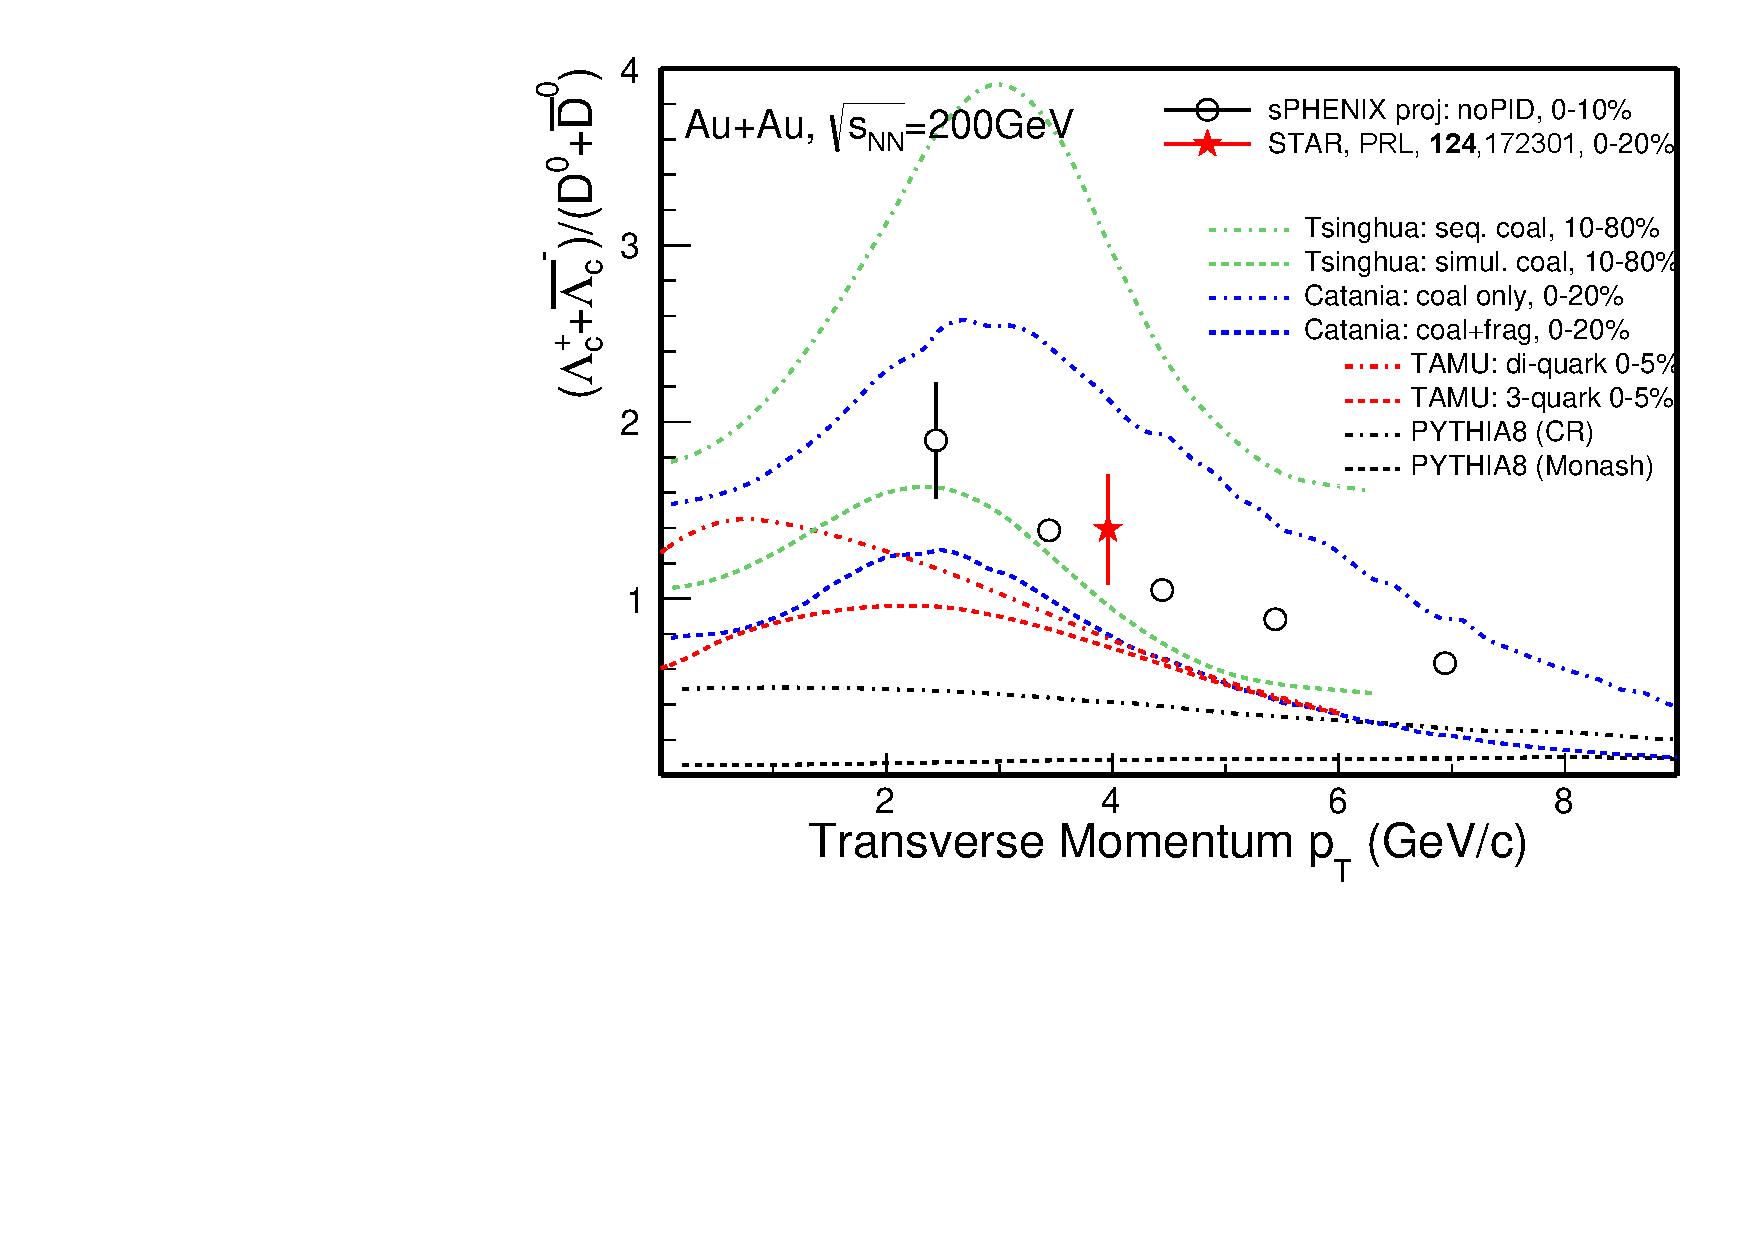
\includegraphics[width=0.48\textwidth]{figs/LcD0_proj_0_10_24B_Update.pdf}
% \caption{Projected statistical uncertainties of $\lambda_c$ to $D^0$ ratio.}
% \label{fig:HF-Lc}
% \end{figure}

\begin{figure}[htbp]
\begin{center}
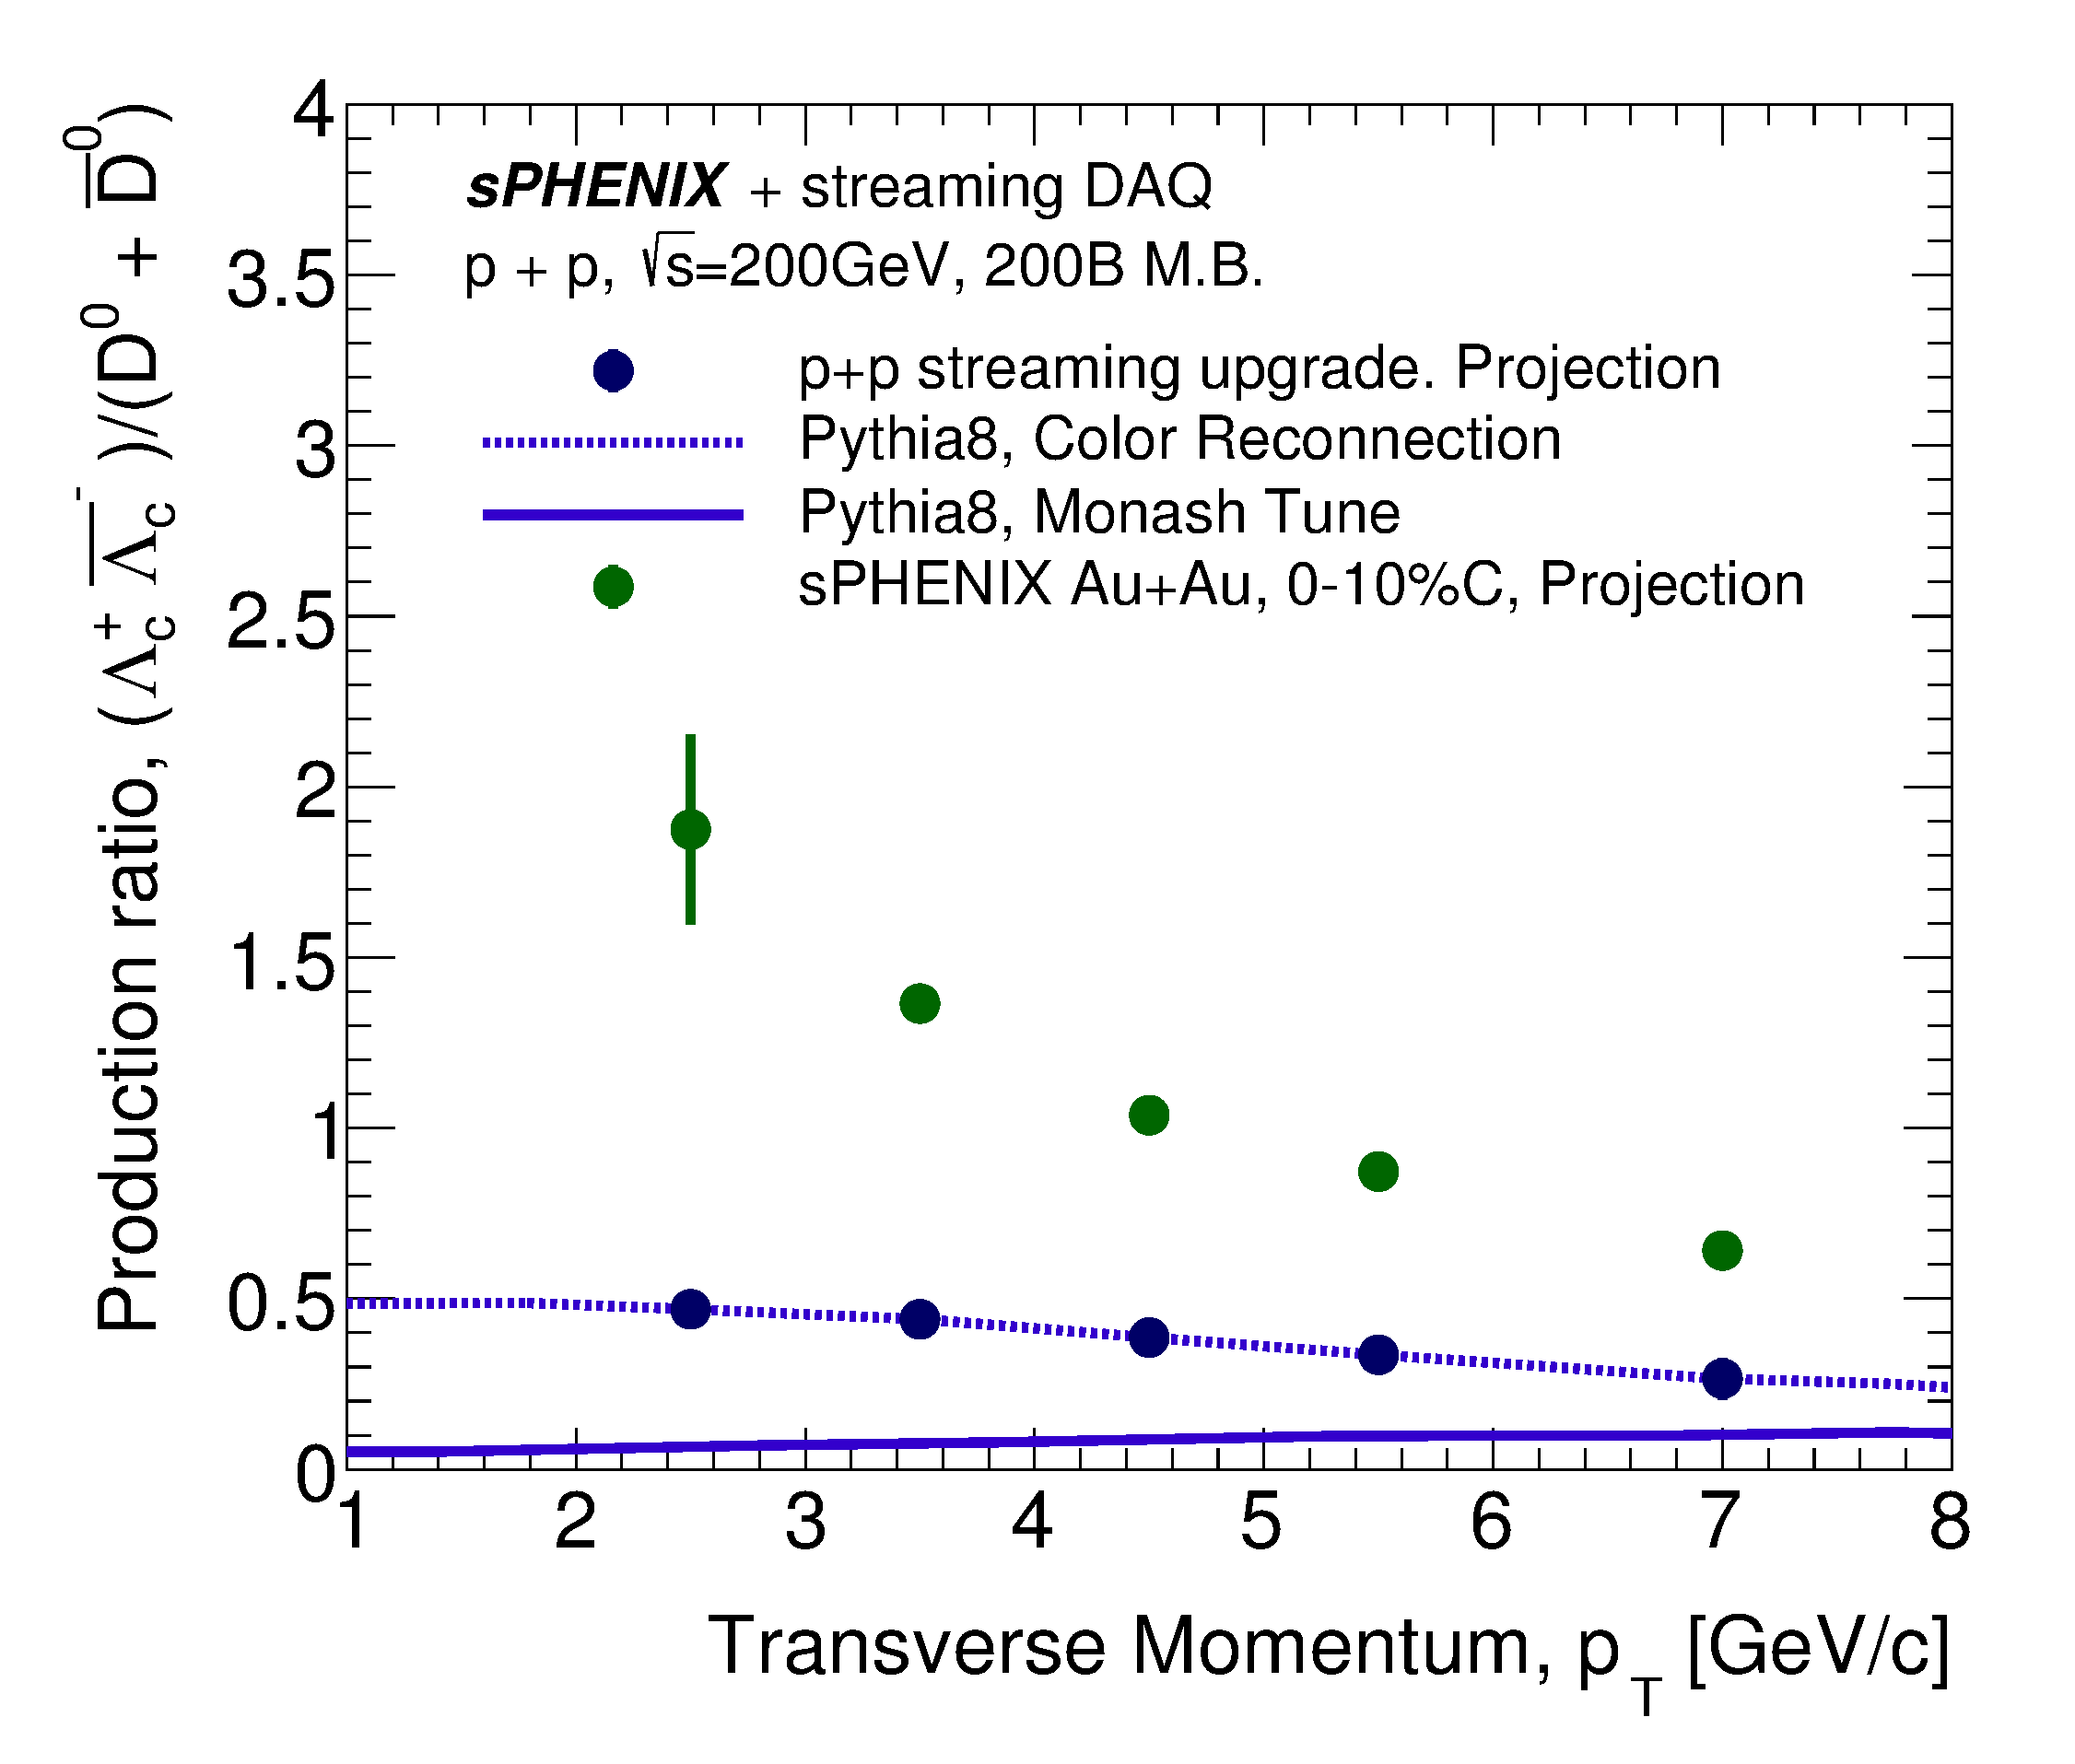
\includegraphics[width=.49\linewidth]{figs/RAA_DB_theory_root_LcD0Ratio_pp200B.pdf}
% 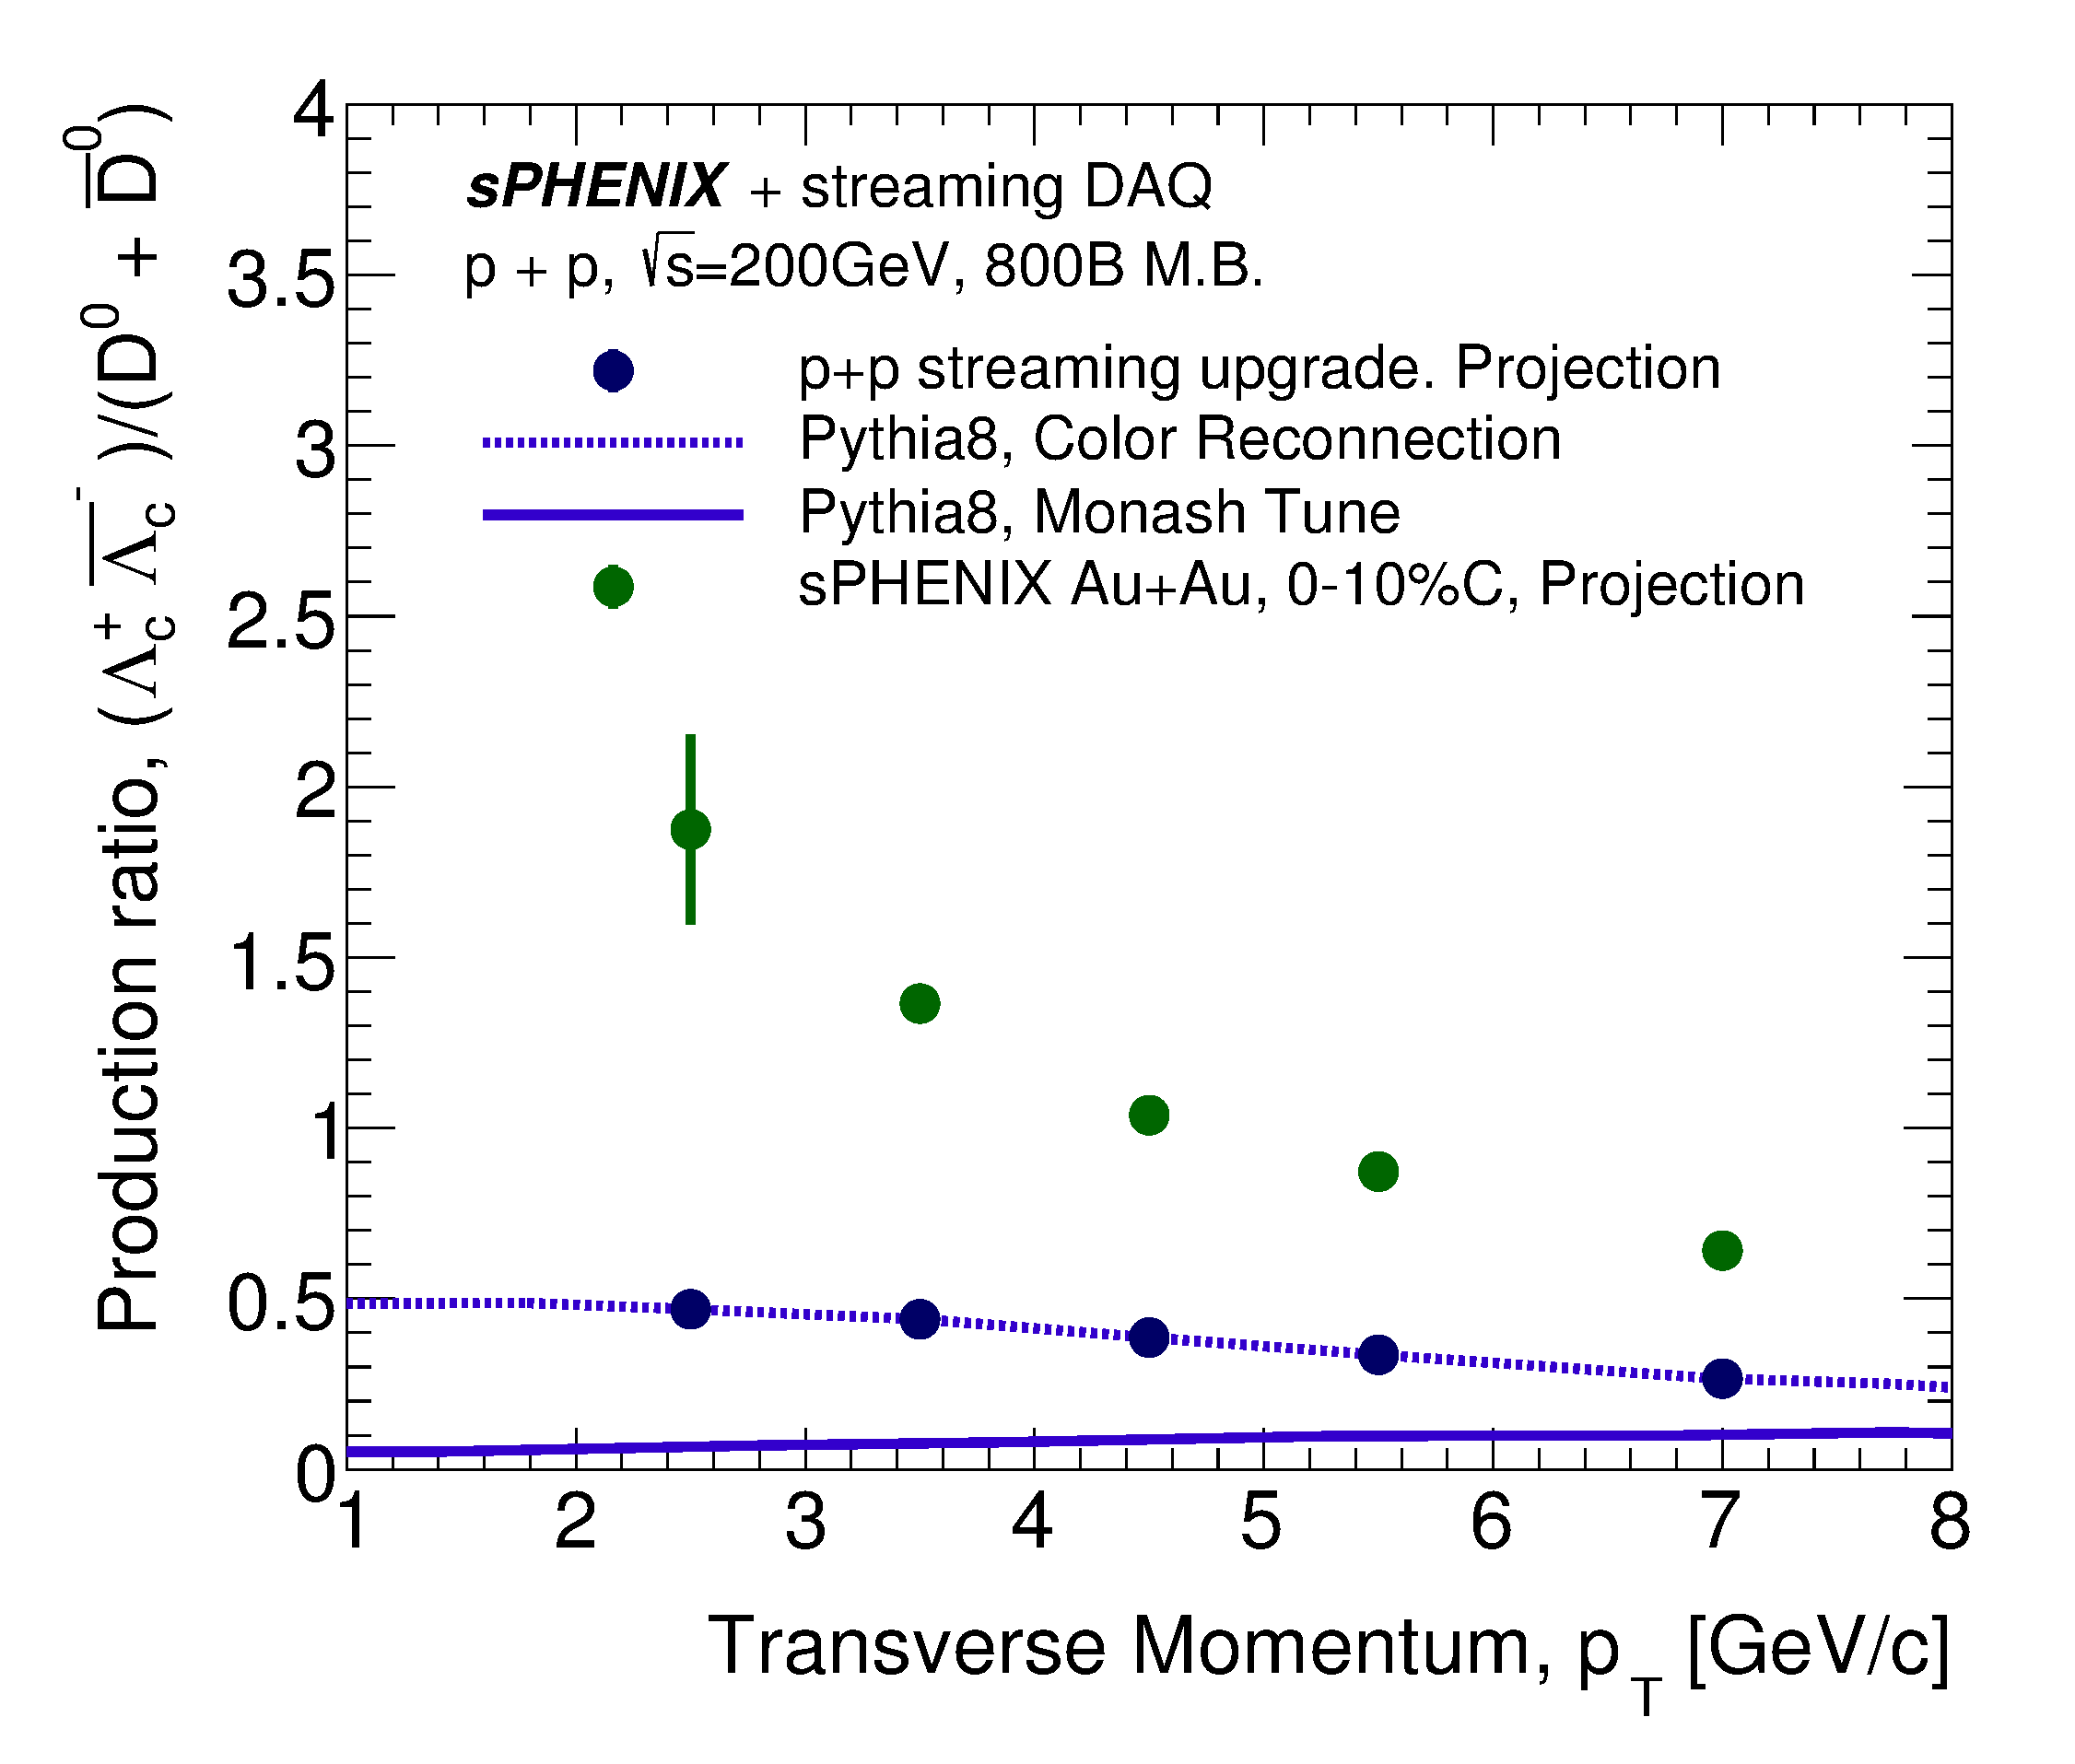
\includegraphics[width=.49\linewidth]{figs/RAA_DB_theory_root_LcD0Ratio.pdf}
\caption{(need STAR published point) Statistical projections of $\Lambda_c/D$ ratio for Year-2 data taking.}
\label{fig:Lc-D0}
\end{center}
\end{figure}



Recent RHIC and LHC data indicate significant enhancements of the
$\lambda_c$ baryon to $D^0$ meson production ratio in \pp,  \pA and
\aa  collisions~\cite{something}. However, the reference $\Lambda_c/D$
ratio in the \pp collision is missing at the RHIC energies, and the
current model predictions differ significantly. As shown in
Figure~\ref{fig:Lc-D0}, this upgrade will enable the first measurement
of the $\Lambda_c/D$ in \pp collisions at RHIC and provide the
critically missing link to quantitatively understand the enhancement
of the charmed baryon/meson production ratio and therefore charm
hadronization in the QGP~\cite{something}.  


 





\section{Cold QCD Physics}
\label{sec:ColdQCD}

The sPHENIX detector, designed to study the QGP with jet, photon and
heavy flavor probes, and with its trigger capabilities and high DAQ
rate capabilities, will provide key opportunities for cold QCD
measurements. These include a broad range of physics measurements with
transversely polarized beams and studies of transverse momentum
effects and hadronization in \pp and \pA collisions.   

%The main emphasis of the RHIC Spin program has been measurements of the gluon polarization in longitudinally polarized proton collisions. RHIC experiments discovered a significant gluon polarization in the gluon momentum fraction range $x>0.05$. Even with the future EIC data expected to precisely measure $\Delta G$ in the lower x region, RHIC data will remain a significant contributor at $x>0.05$. However, any significant improvement of $\Delta G$ measurements, compared to existing RHIC data (published and being analyzed), requires significant integrated luminosity (at least a few hundred pb$^{-1}$), which is not anticipated in the sPHENIX 3-year running scenario. Therefore in this document we focus on the measurements with transversely polarized beams.

\subsection {Transverse Spin Measurements}

In recent years, transverse spin phenomena have gained substantial
attention. The nature of significant transverse single spin
asymmetries (TSSAs) in hadron collisions, discovered more than 40
years ago at low center of mass energy ($\sqrt{s}=4.9$~GeV), and then
confirmed at higher energies up to $\sqrt{s}=500$~GeV and $p_T \sim
7$~GeV/$c$ at RHIC, has not yet been fully understood. Different
mechanisms are suggested to explain such asymmetries, involving
initial-state and final-state effects, in the collinear or
transverse-momentum-dependent (TMD) framework. These descriptions have
deep connections to nucleon partonic structure and parton dynamics
within the nucleon, as well as spin-momentum correlations in the
process of hadronization. 

The TSSAs in direct photon and heavy flavor production probe the gluon
dynamics within a transversely polarized nucleon, described by the
tri-gluon correlation function in the collinear twist-3 framework,
which is connected with the gluon Sivers TMD parton distribution
function (PDF), thus far poorly constrained. The Sivers function
correlates the nucleon transverse spin with the parton transverse
momentum. 

The projected uncertainties for the midrapidity direct photon TSSAs compared to theoretical calculations are shown in Figure~\ref{fig:AN_dp}. The direct photon sample here will be collected with an EMCal-based high-energy cluster trigger. 
%Asymmetry measurements in $D^0$ meson production through its hadronic decay will be done from a minimum bias (MB) sample collected with streaming readout. Figure~\ref{fig:AN-D0} shows the projected uncertainties for such a measurement.
The new capability of the sPHENIX streaming DAQ (detailed in
Section~\ref{sec:streaming_readout}) enables a high precision
measurement of $D^0$ TSSA in the mid-rapidity region as shown in
Figure~\ref{fig:AN-D0}.  
%This observable is a unique probe of the twist-3 tri-gluon correlation function and gluon Sievers effect in the polarized proton, which opens a new window into the dynamics of gluons in hadrons [Reference to be updated]. 

\begin{figure}[htbp]
\centering
\includegraphics[width=0.60\textwidth]{figs/AN_dp_sphenix.pdf}
\caption{Projected statistical uncertainties for direct photon $A_N$.}
\label{fig:AN_dp}
\end{figure}

\begin{figure}[htbp]
\begin{center}
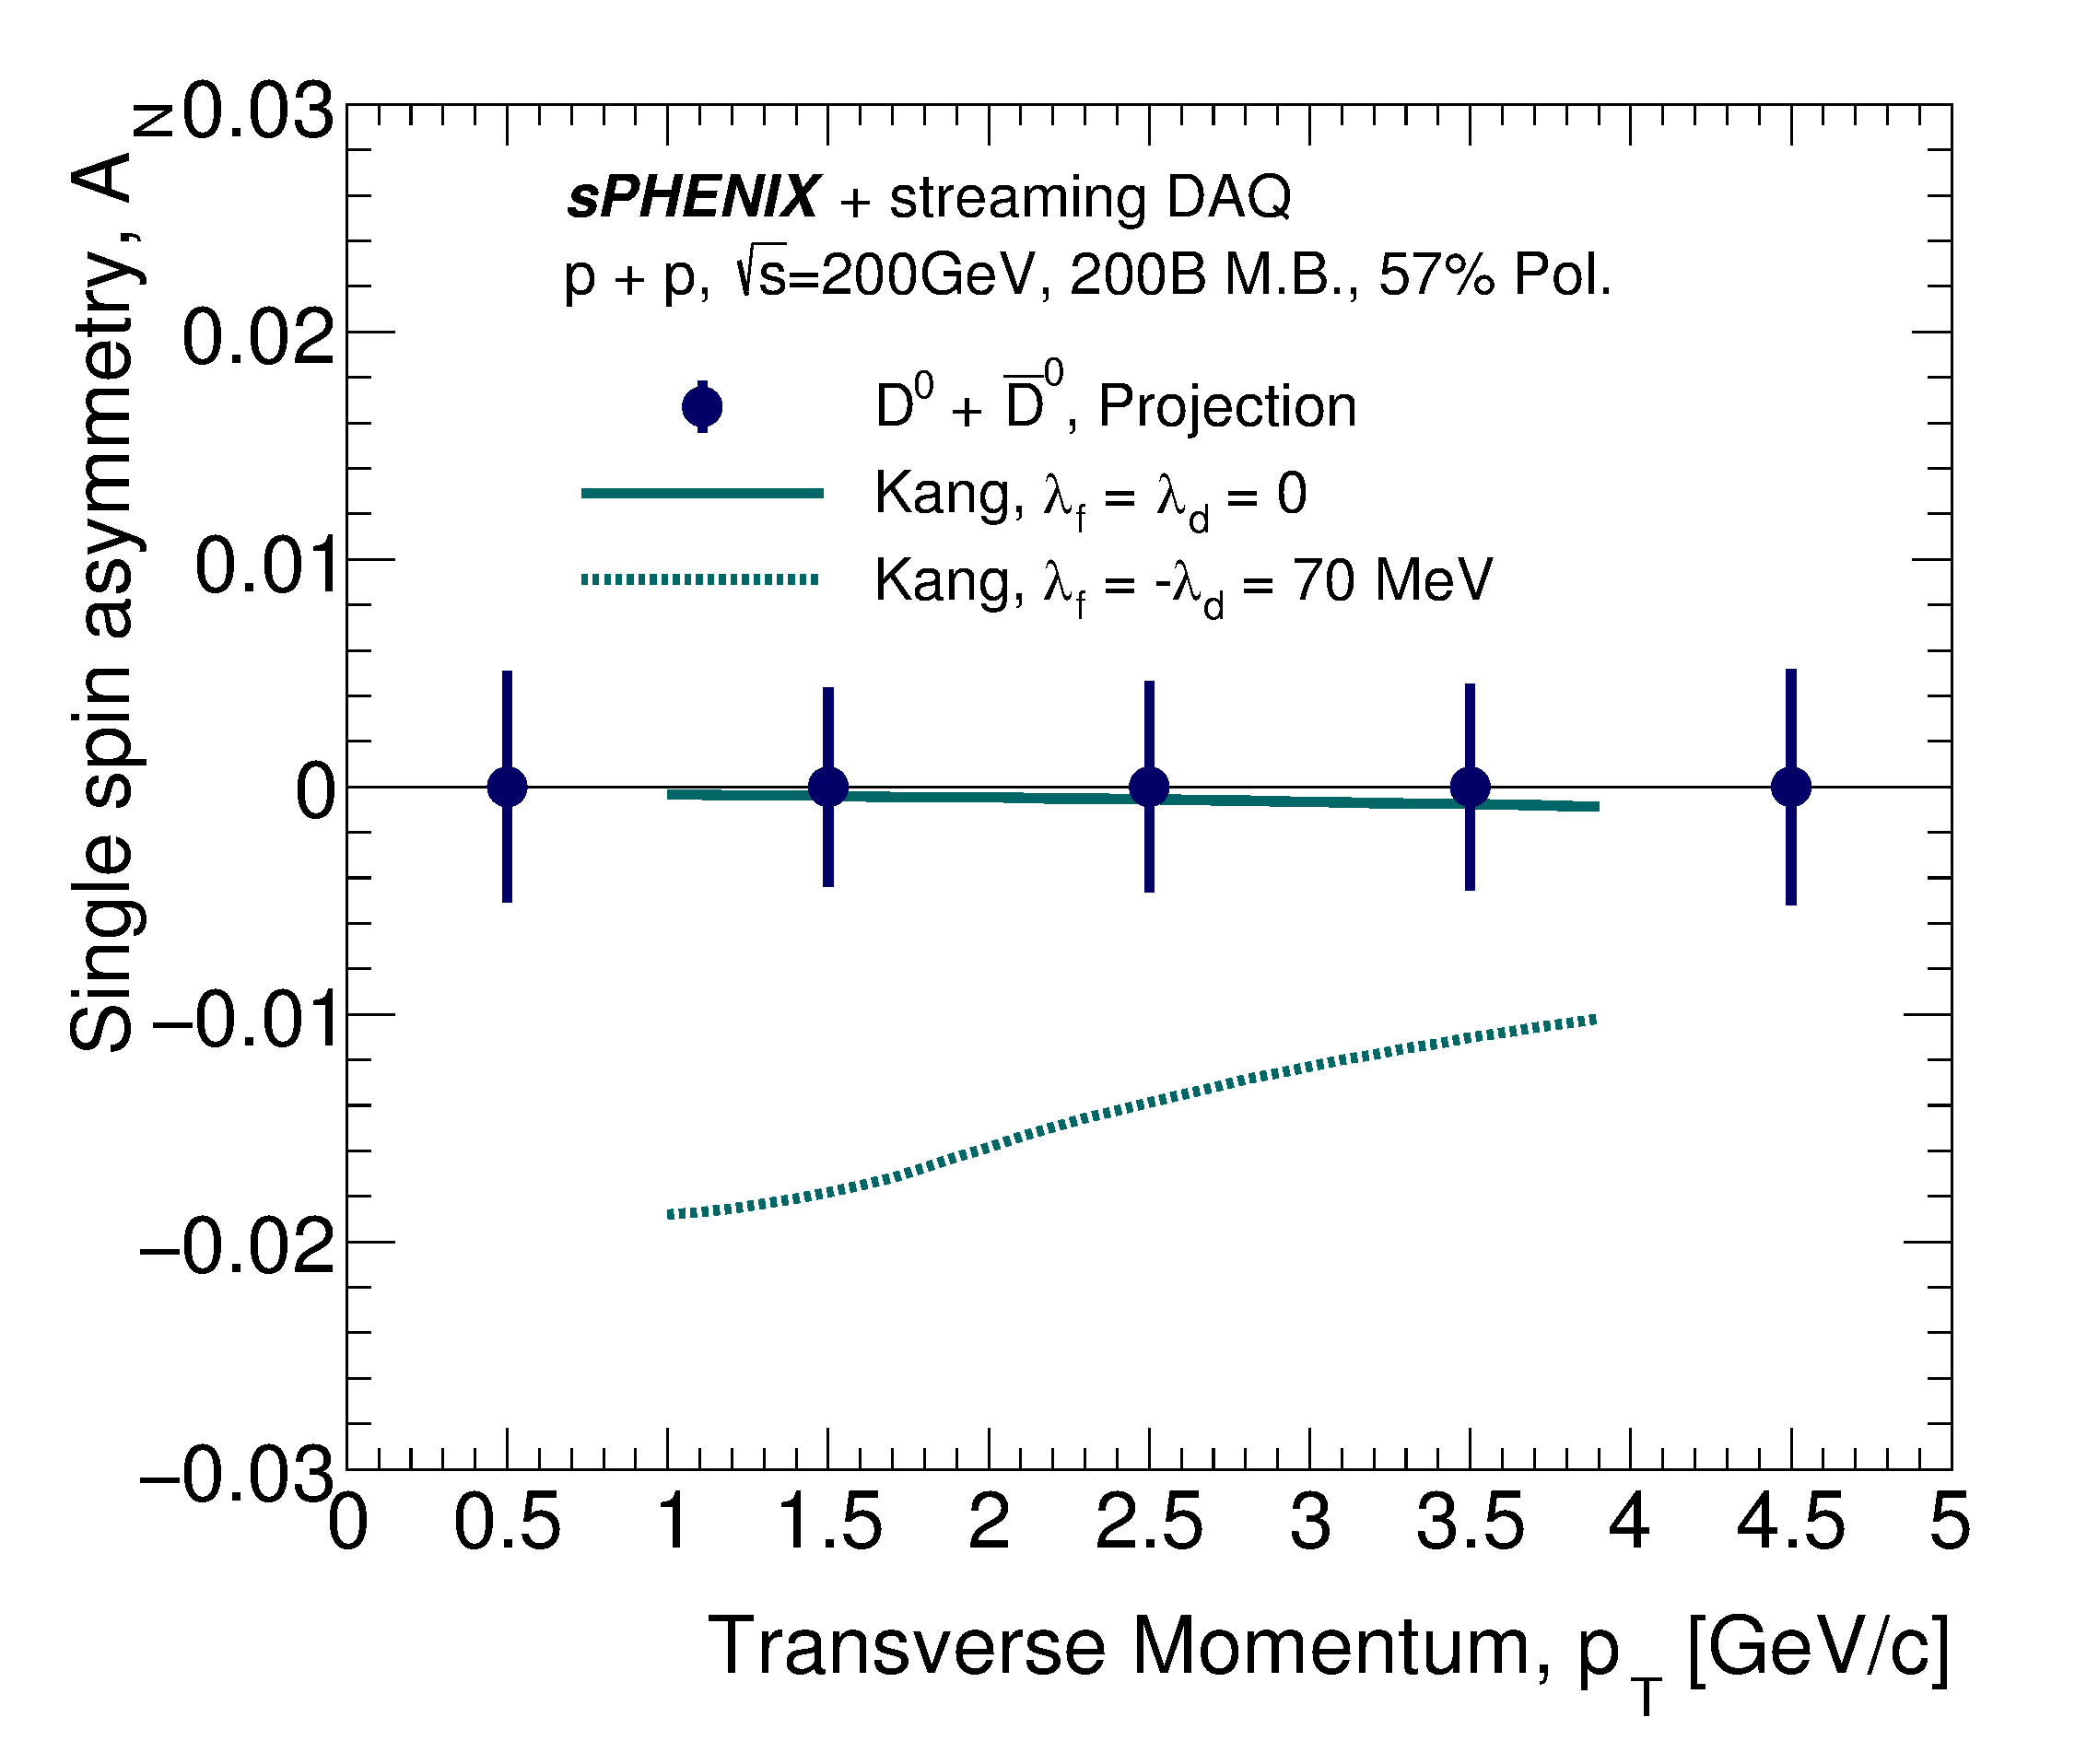
\includegraphics[width=.49\linewidth]{figs/RAA_DB_theory_root_AN_D0D0bar_pp200B.pdf}
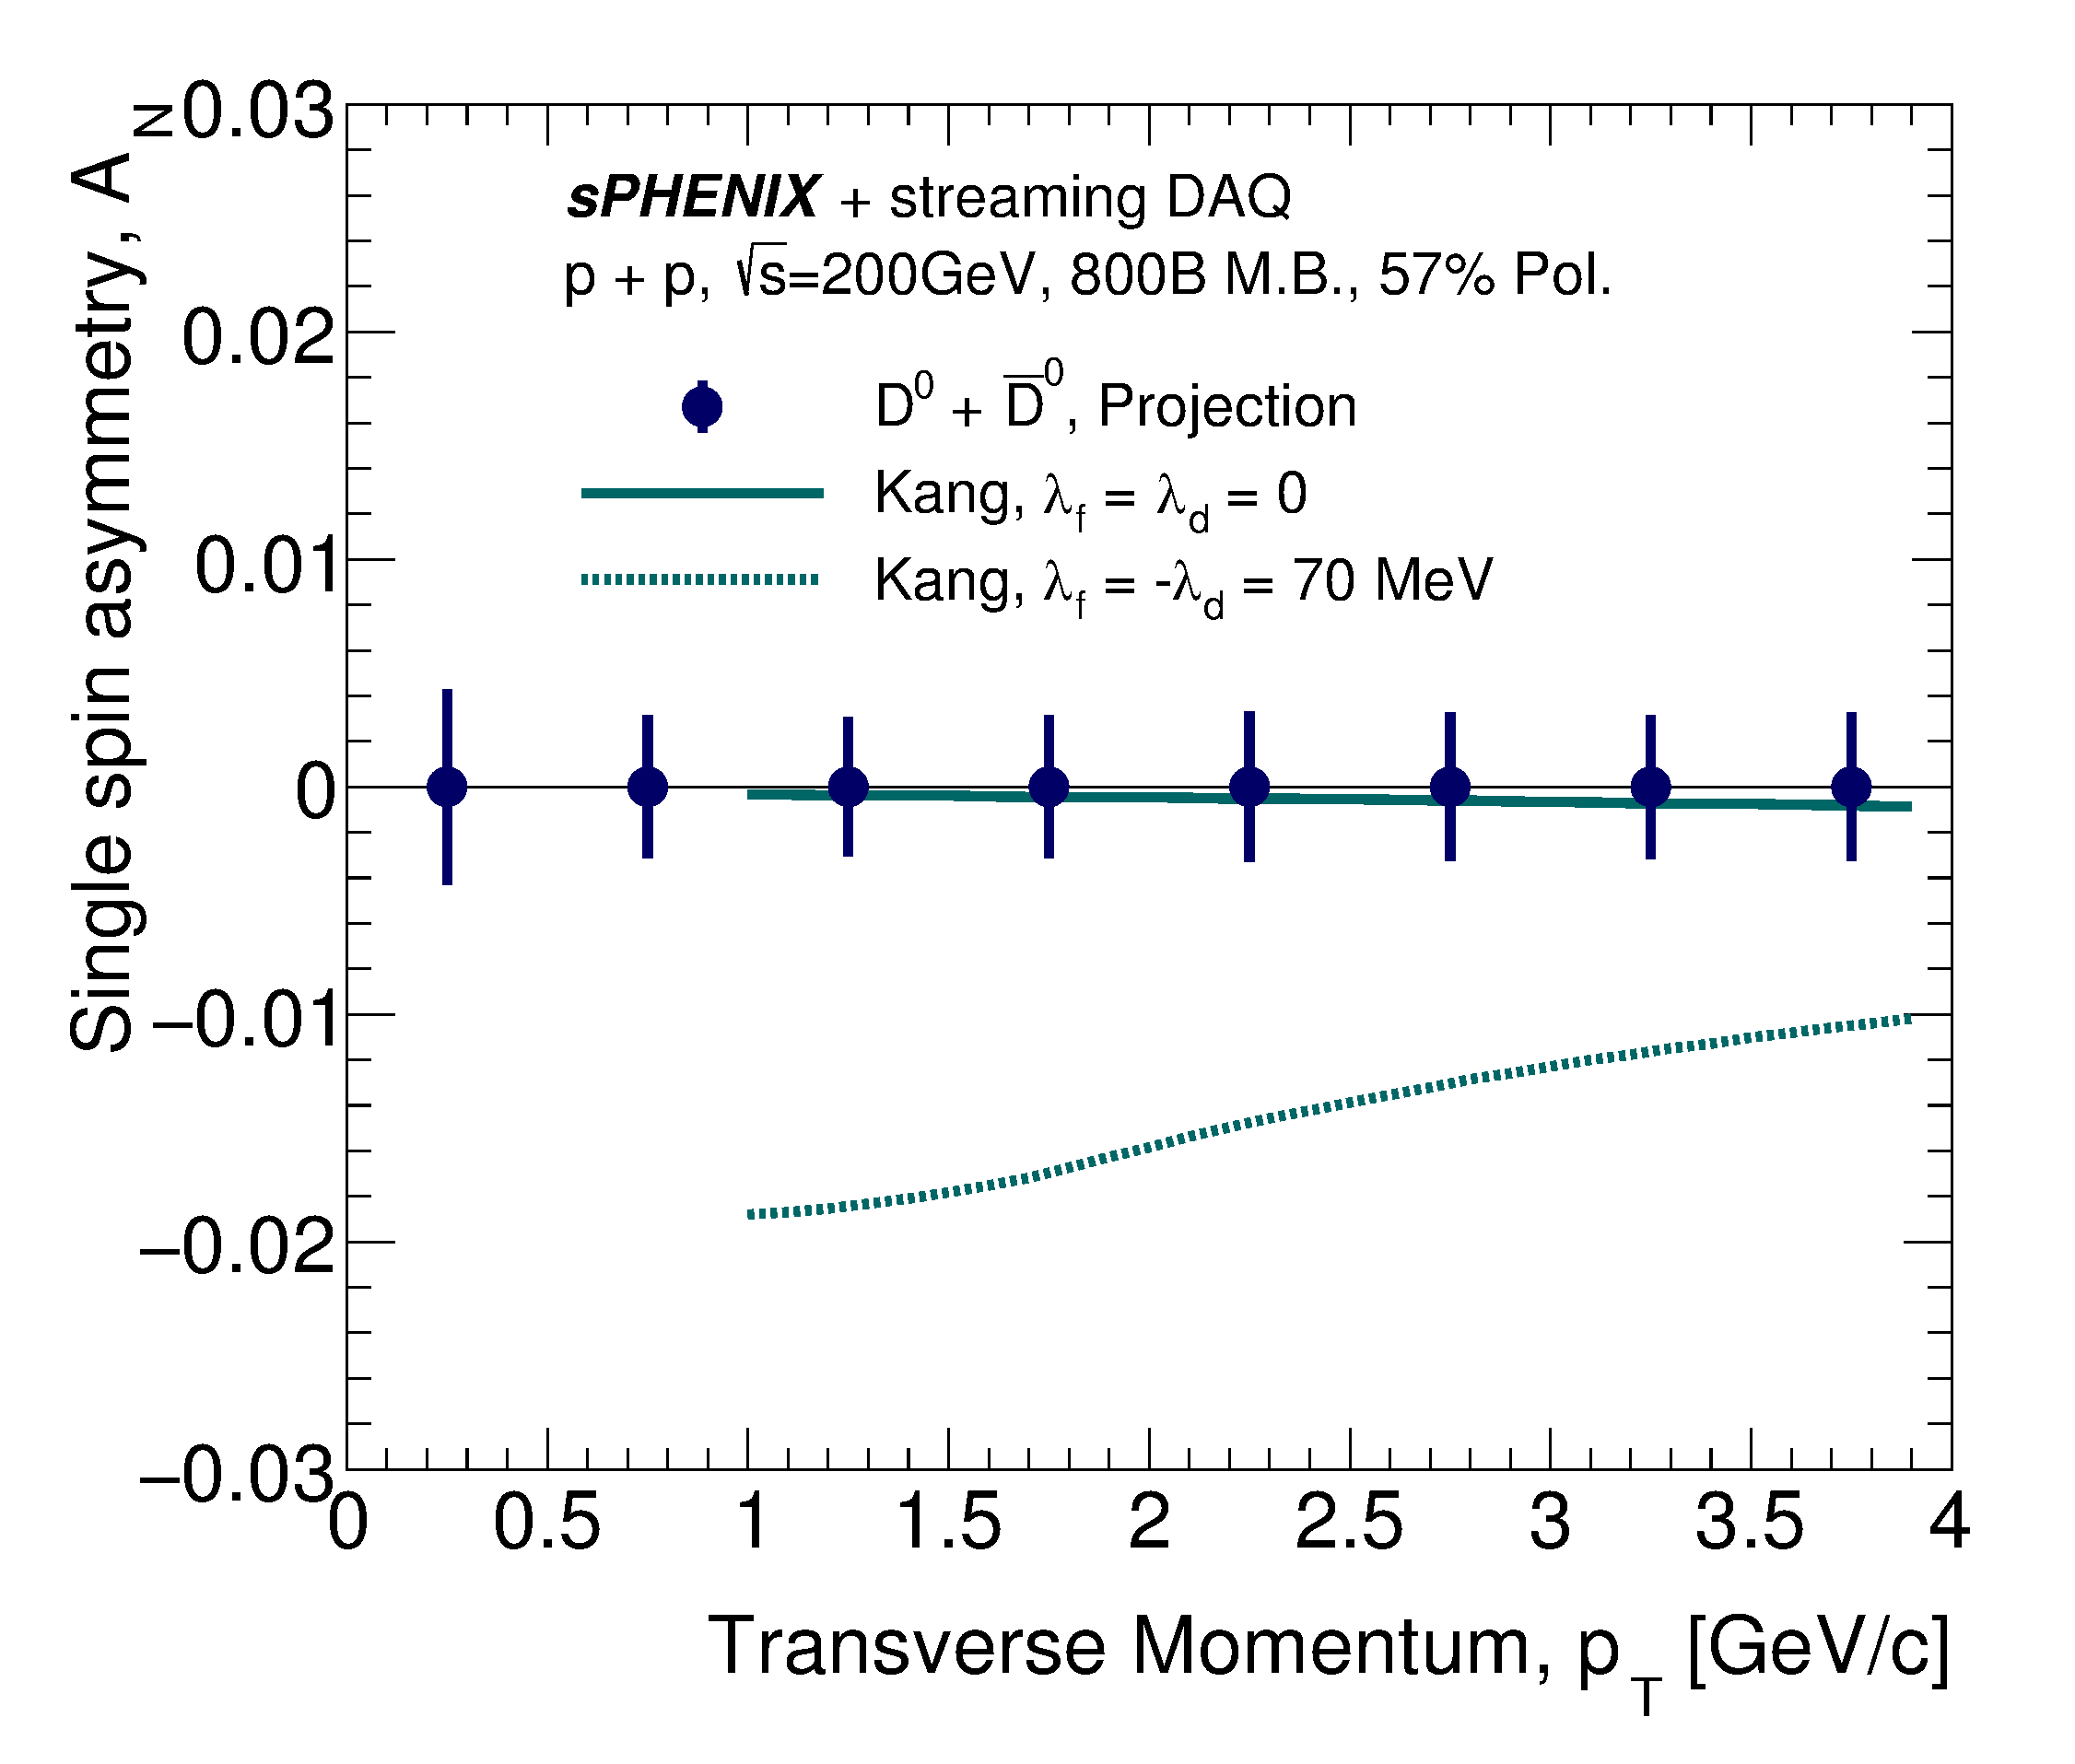
\includegraphics[width=.49\linewidth]{figs/RAA_DB_theory_root_AN_D0D0bar.pdf}
\caption{[To be updated with lumi numbers] Statistical projections of
  transverse spin asmmetry for the $D^0$ mesons for Year-2 and Year
  2+4 data taking.} 
\label{fig:AN-D0}
\end{center}
\end{figure}

Another interesting channel related to the Sivers effect is the inclusive jet TSSA, which has not yet been measured at central rapidity. sPHENIX can provide high precision measurements with uncertainties on the level of a few times $10^{-4}$. While the opposite sign contribution of up and down quarks to Sivers asymmetry is expected to suppress the measured TSSA, tagging the leading hadron charge will preferentially enhance the contribution from fragmenting up or down quarks, and therefore will enable the flavor-separated measurements in the central rapidity kinematics.

Dijet measurements allow for direct access to parton intrinsic transverse momentum $k_T$. Again, charged tagging will enhance the effect from either up or down quarks, which otherwise will be essentially cancelled out. Recent STAR preliminary results showed a nonzero effect for charge-tagged jets. sPHENIX as a dedicated detector for jet and photon measurements is expected to significantly contribute to these measurements and to extend it to photon-jet measurements, which essentially isolate the quark-gluon scattering process at leading order, thus giving access to the gluon Sivers effect.

Another possible origin of the observed TSSAs is the Collins mechanism, which correlates the transverse polarization of a fragmented quark to the angular distribution of hadrons within a jet. This gives access to the transversity distribution in the proton, which can be interpreted as the net transverse polarization of quarks within a transversely polarized proton. Along with the unpolarized PDF and helicity PDF, transversity is one of three leading-twist PDFs, least known at the moment. The integral in $x$ over the valence quark transversity distribution defines the tensor charge, a fundamental value calculable in lattice QCD, therefore enabling the crucial comparison of experimental measurements with ab-initio theoretical calculations.

Measuring angular distributions of dihadrons in the collisions of
transversely polarized protons, couples transversity to the so-called
``interference fragmentation function'' (IFF) in the framework of
collinear factorization. The IFF describes a correlation between the
spin of an outgoing quark and the angular distribution of a hadron
pair that fragments from that quark.  A comparison of the transversity
signals extracted from the Collins effect and IFF measurements will
explore questions about universality and factorization breaking. 

The first nonzero Collins and IFF asymmetries in \pp collisions have
been observed by the STAR collaboration at midrapidity and shown to be
invaluable to constrain the transversity distribution. sPHENIX, with
its excellent hadron and jet calorimetric trigger capabilities coupled
with its high-rate DAQ capabilities, is expected to deliver
high-statistics samples for both Collins and IFF
asymmetries. sPHENIX's capability to collect a significant 
data sample with streaming readout will allow us to extend the charged
dihadron measurements for IFF asymmetries from the barrel region
($|\eta|<1$) to more forward kinematics up to $\eta=2$.  
%Fig.* shows projected uncertainties for IFF asymmetries [hopefully we'll get them].


\subsection {Transverse Spin: \pp vs \pA}

$p\uparrow$$+$A collisions at RHIC provide unique opportunities to
study spin effects in a nuclear environment. These studies may provide
new insights into the origin of the observed TSSAs and a unique tool
to investigate the rich phenomena behind TSSAs in hadronic
collisions. TSSAs measured in polarized $p$+A collisions moreover
offer a new approach to studying small-system collisions, in which
numerous surprising effects have been observed in recent years. 

First RHIC results from the 2015 RHIC run showed a puzzling evolution
of the TSSA from \pp to \pAl and then \pAu. While STAR's
preliminary result for $\pi^{0}$ asymmetry in forward rapidity (with
$0.2<x_F<0.7$) showed no significant nuclear dependence, PHENIX's
positively charged hadron asymmetries in the intermediate rapidity
range (with $0.1<x_F<0.2$) discovered a strong nuclear dependence in
the TSSA, from $A_N \sim 0.03$ in $p+p$ collisions to a value
consistent with zero in \pAu collisions. No clear explanation for
such a behavior has been offered at the moment. Obviously, more data,
differentiated in $p_T$ and $x_F$, would be highly desirable. sPHENIX
is able to collect much more data in this channel, with fine binning,
which is expected to provide crucial information on the nature of
TSSAs in hadronic collisions and on understanding of the spin probe---
nucleus interaction, a novel topic directly associated with RHIC's
unique ability to collide polarized protons with nuclei. 

Figure~\ref{fig:AN_h} shows the projected uncertainties for sPHENIX,
based on MB data collected with the streaming readout. The sPHENIX
tracking system will provide us with charged hadron measurements in
the pseudorapidity range up to $\eta=2$, which overlaps with the
PHENIX range, where the strong nuclear effect was observed
($1.2<\eta<2.4$). 

\begin{figure}[htbp]
\centering
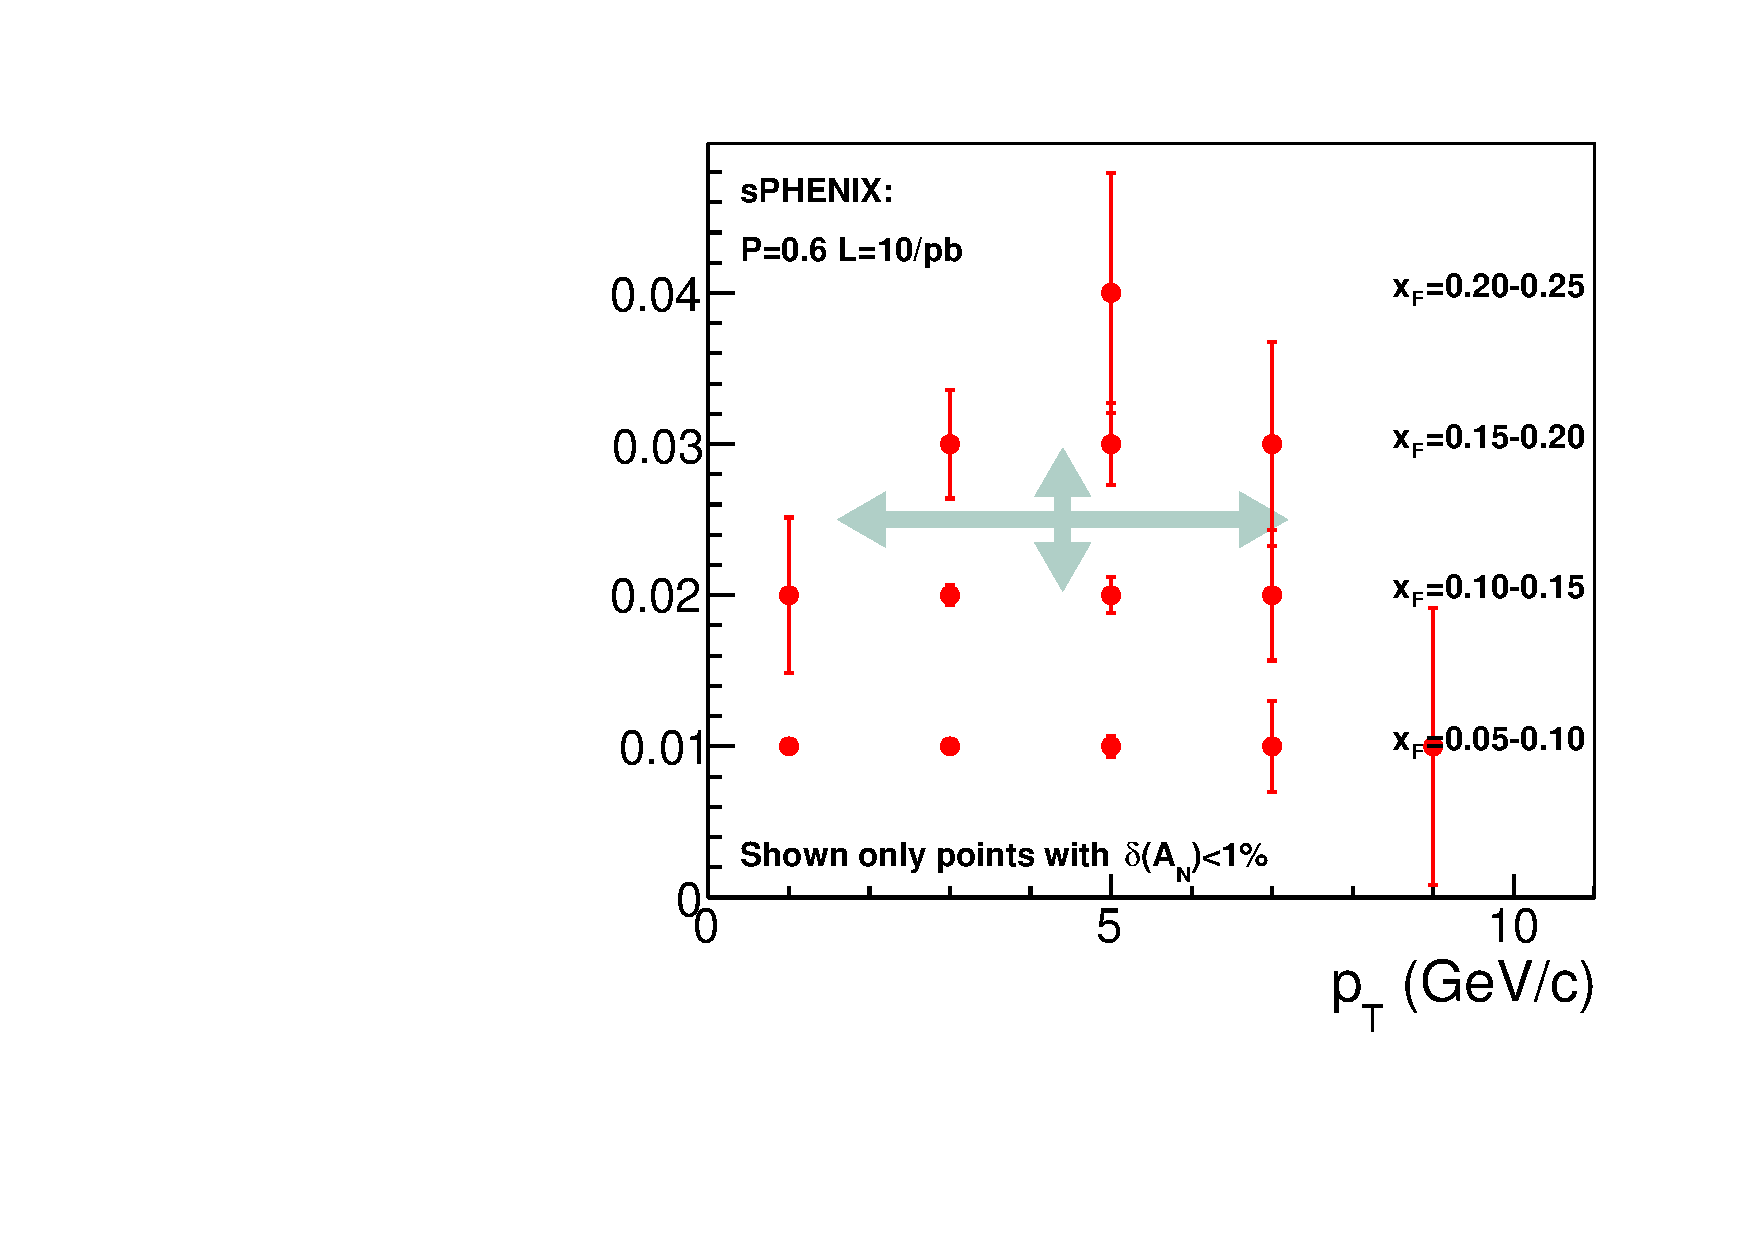
\includegraphics[width=0.60\textwidth]{figs/sphenix_han.pdf}
\caption{Projected statistical uncertainties for $h^{+}$ $A_N$ in
  \pp collisions, for data collected with streaming readout; similar
  uncertainties are expected from \pAu data; green arrows indicate
  the stat. uncertainty and the $p_T$ coverage of the PHENIX data
  point (with $0.1<x_F<0.2$).} 
\label{fig:AN_h}
\end{figure}

The other measurements (e.g. Collins and IFF asymmetries) will also be
compared between \pp and \pA systems and may potentially bring new
surprises. 


\subsection {Unpolarized Measurements}

A number of cold QCD measurements that do not require beam
polarization are planned in \pp and \pA collisions. Hadronization
studies will be performed with hadron-in-jet measurements,
multidifferential in momentum fraction $z$ of the jet carried by the
produced hadron, in the transverse momentum $j_T$ of the hadron with
respect to the jet axis, and in the angular radial profile $r$ of the
hadron with respect to the jet axis. This includes studies for both
light quark and heavy quark hadrons. Comparison of \pp and pA
collisions will provide information on the nuclear modification of
hadronization processes. Measurements performed by PHENIX of
nonperturbative transverse momentum effects and their nuclear
modifications in back-to-back dihadron and photon-hadron correlations,
will be extended to dijet and photon-jet measurements in sPHENIX.
These measurements will help to separate the effects associated with
intrinsic parton momentum $k_T$ in the nucleon or nucleus and
fragmentation transverse momentum $j_T$. These correlation
measurements may also help to probe theoretically predicted
factorization breaking effects within the
transverse-momentum-dependent framework. Upsilon and \jpsi
polarization measurements will shed further light on heavy quarkonium
production mechanisms. 
